Após a execução do Script de codificação, os dados obtidos são armazenado
em um arquivo CSV. Com os resultados finais, outro script em \textit{Python} é
executado, onde ele cria um gráfico com estes dados. Abaixo estão os resultados
obtidos.

A análise dos gráficos gerados para as sequências testadas permite observar o comportamento 
do \acrshort{LCEVC} em diferentes condições de codificação. Foram analisadas dois
codificadores: \acrshort{AVC} e \acrshort{VVC}, com e sem o uso do \acrshort{LCEVC} 
como camada de aprimoramento.

No geral, os gráficos \acrshort{PSNR} x \textit{Bitrate} permitem avaliar a eficiência da
compressão, considerando que uma melhor relação é obtida quando se atinge maior qualidade
(\acrshort{PSNR}) com menor taxa de bits (\textit{bitrate}). A seguir, apresenta-se uma
análise detalhada por cenário. Para alguns resultados, se um vídeo em \acrshort{LCEVC} 
resultou em um valor muito alto para o \textit{bitrate}, onde fique distante dos valores
do codificador base, eles foram omitidos para melhor análise e visualização nos gráficos.

Além disso, para que o gráfico pudesse ficar legível, só foi rotulado o valor de SW2 para
o parâmetro de QP37.

\newpage
\section{AVC}

\subsection{Bosphorus}
\begin{figure}[h]
    \centering
    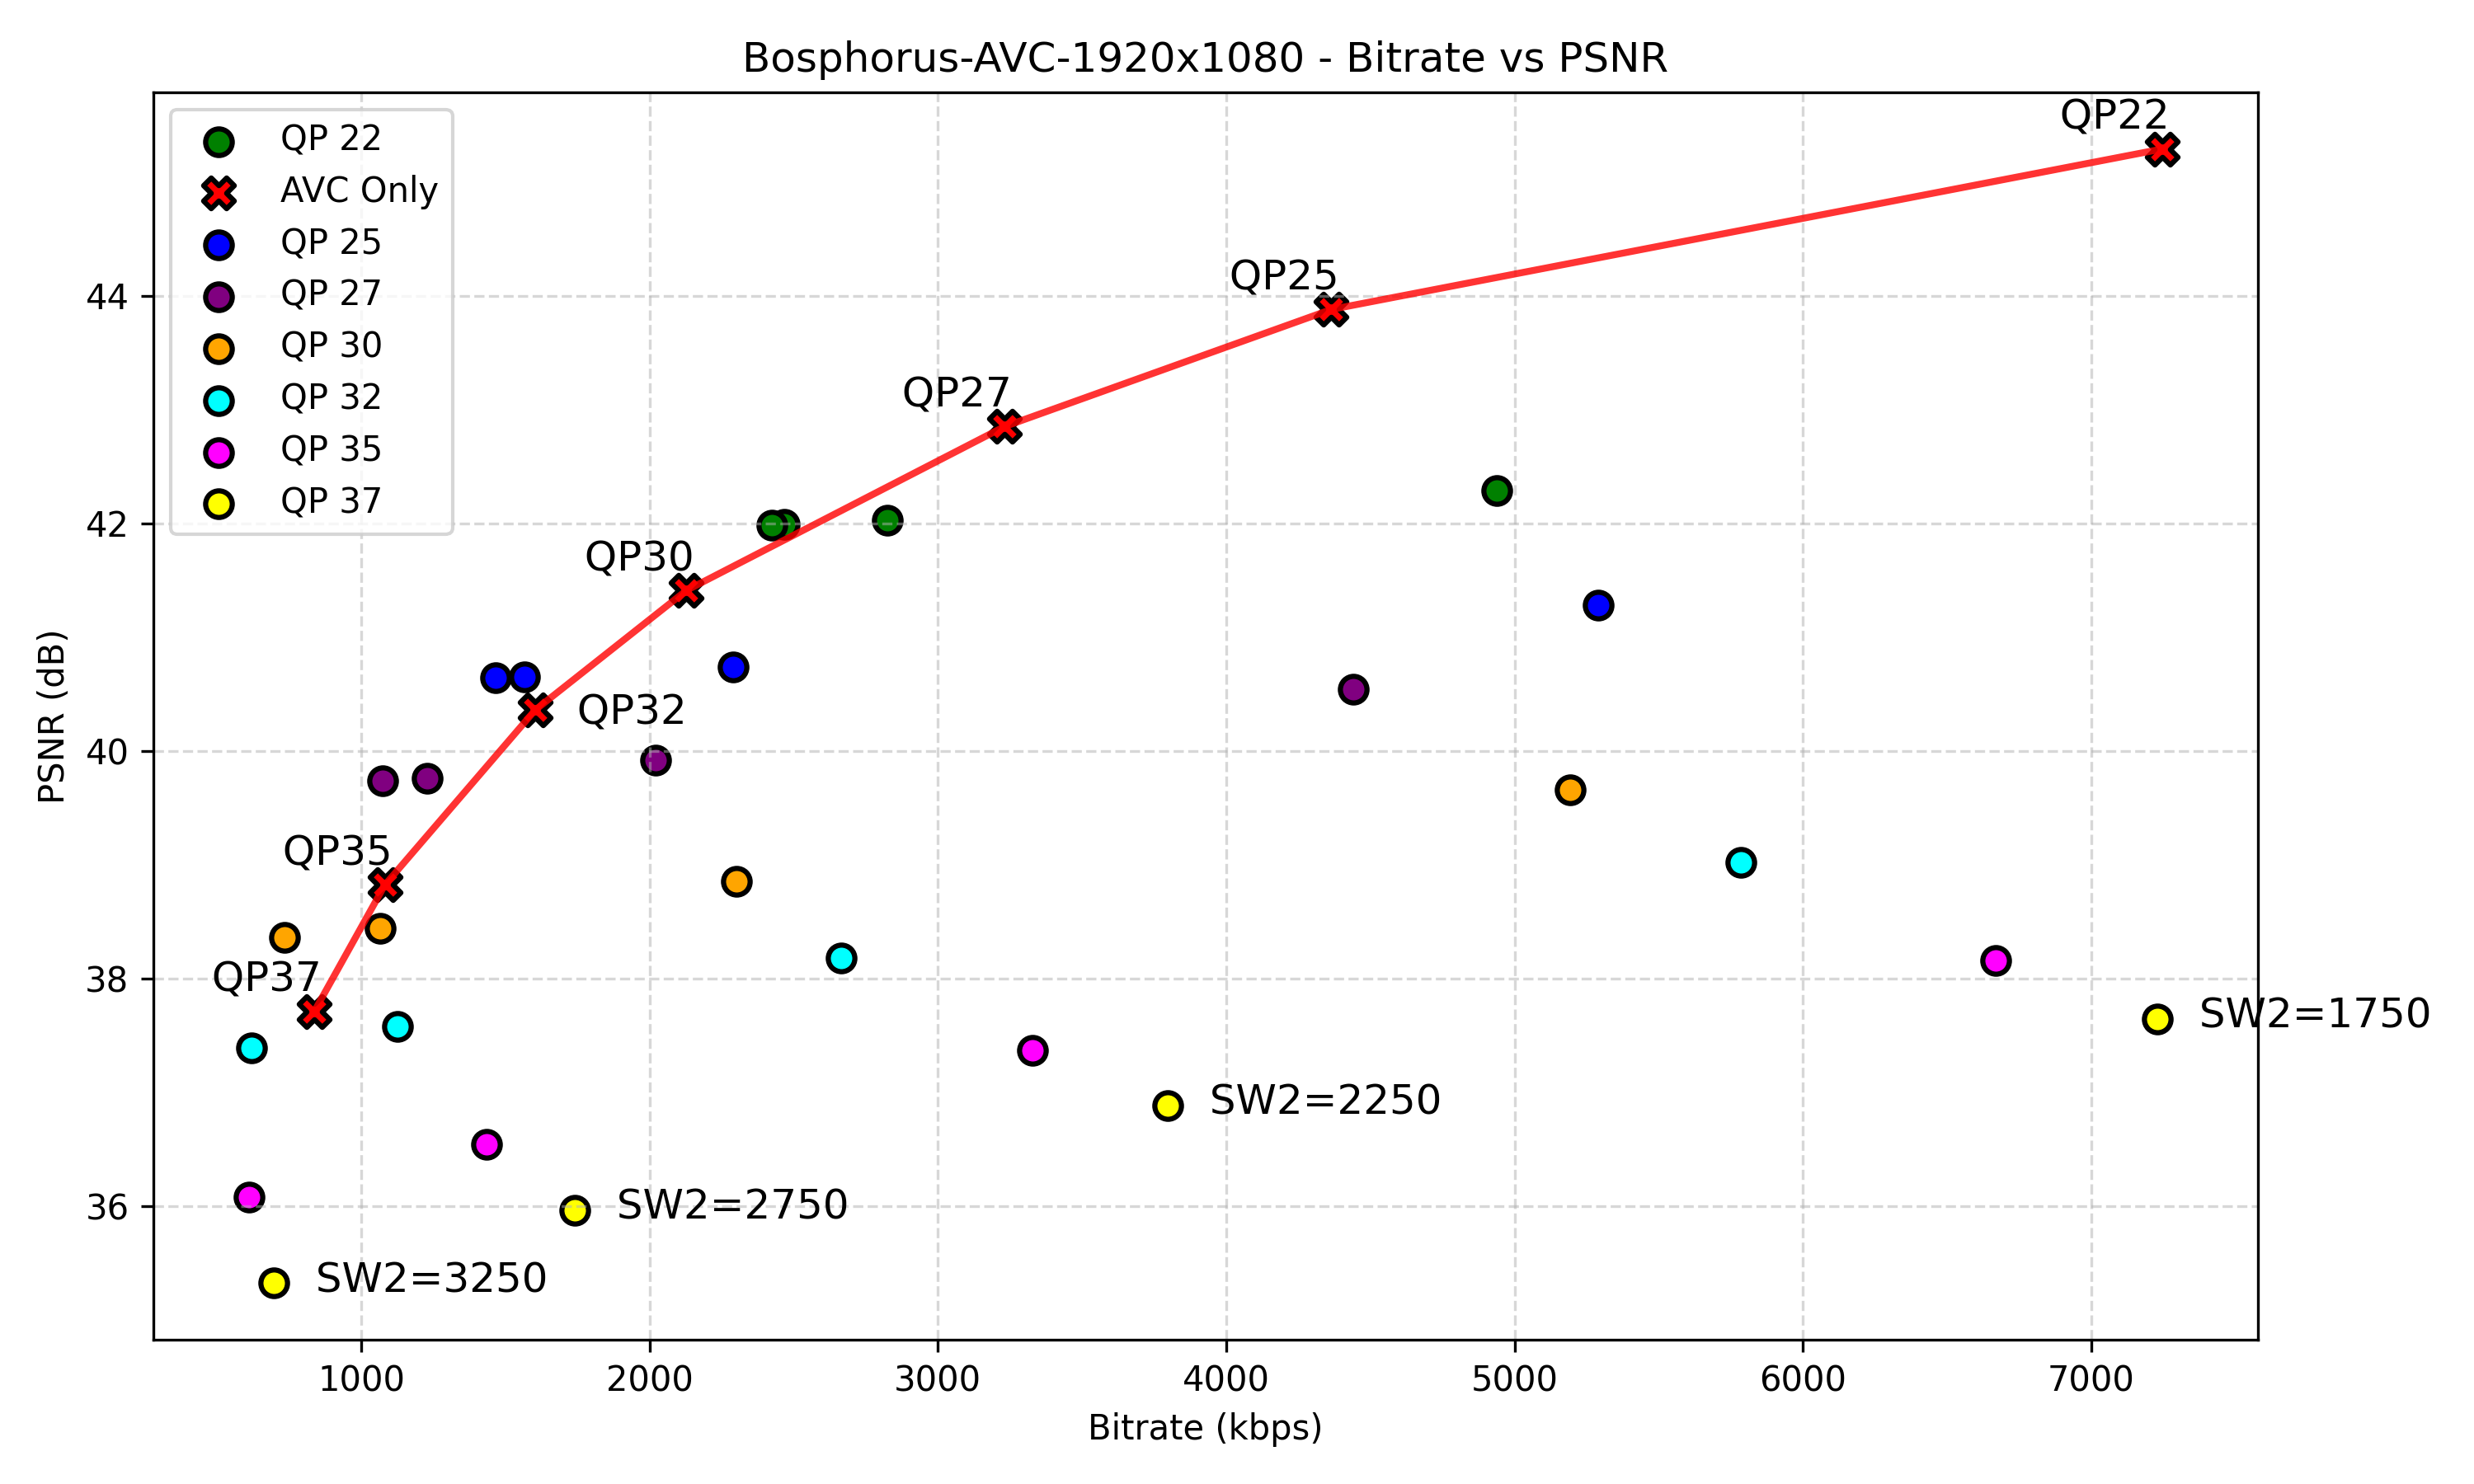
\includegraphics[width=1.0\textwidth]{img/Bosphorus-AVC.png}
    \caption{Resultados para "Bosphorus"\ em \acrshort{AVC}. \cite{uvg_dataset}}
    \label{fig:bosphorus}
\end{figure}

Para a sequência Bosphorus, os resultados revelam que o uso do \acrshort{LCEVC} pode
ser vantajoso em determinados cenários, dependendo dos parâmetros utilizados.

Nos testes com valores baixos de SW2, observou-se que, embora o \acrshort{PSNR} 
alcançado seja alto, os arquivos resultantes apresentam um \textit{bitrate}
superior ao necessário para atingir uma qualidade semelhante utilizando
somente o \acrshort{AVC}. 

Para valores intermediários de SW2, os resultados foram mais promissores. Nestes
casos, o \acrshort{LCEVC} foi capaz de alcançar uma boa relação entre qualidade
e taxa de bits. Nestes casos, embora o \acrshort{PSNR} seja um pouco inferior,
o \acrshort{LCEVC} pode ser interessante em contextos onde a reconstrução visual
seja mais importante que o valor do \acrshort{PSNR}.

Para valores mais altos de SW2, como 2250 por exemplo, a camada de aprimoramento
passou a contribuir muito pouco para a codificação, representando uma proporção
bem pequena do tamanho total do arquivo. Neste caso, o \acrshort{LCEVC} possui
sua codificação comprometida pela perda de qualidade e espaço, tornando estas
configurações pouco vantajosas.

\subsection{ReadySteadyGo}

\begin{figure}[h]
    \centering
    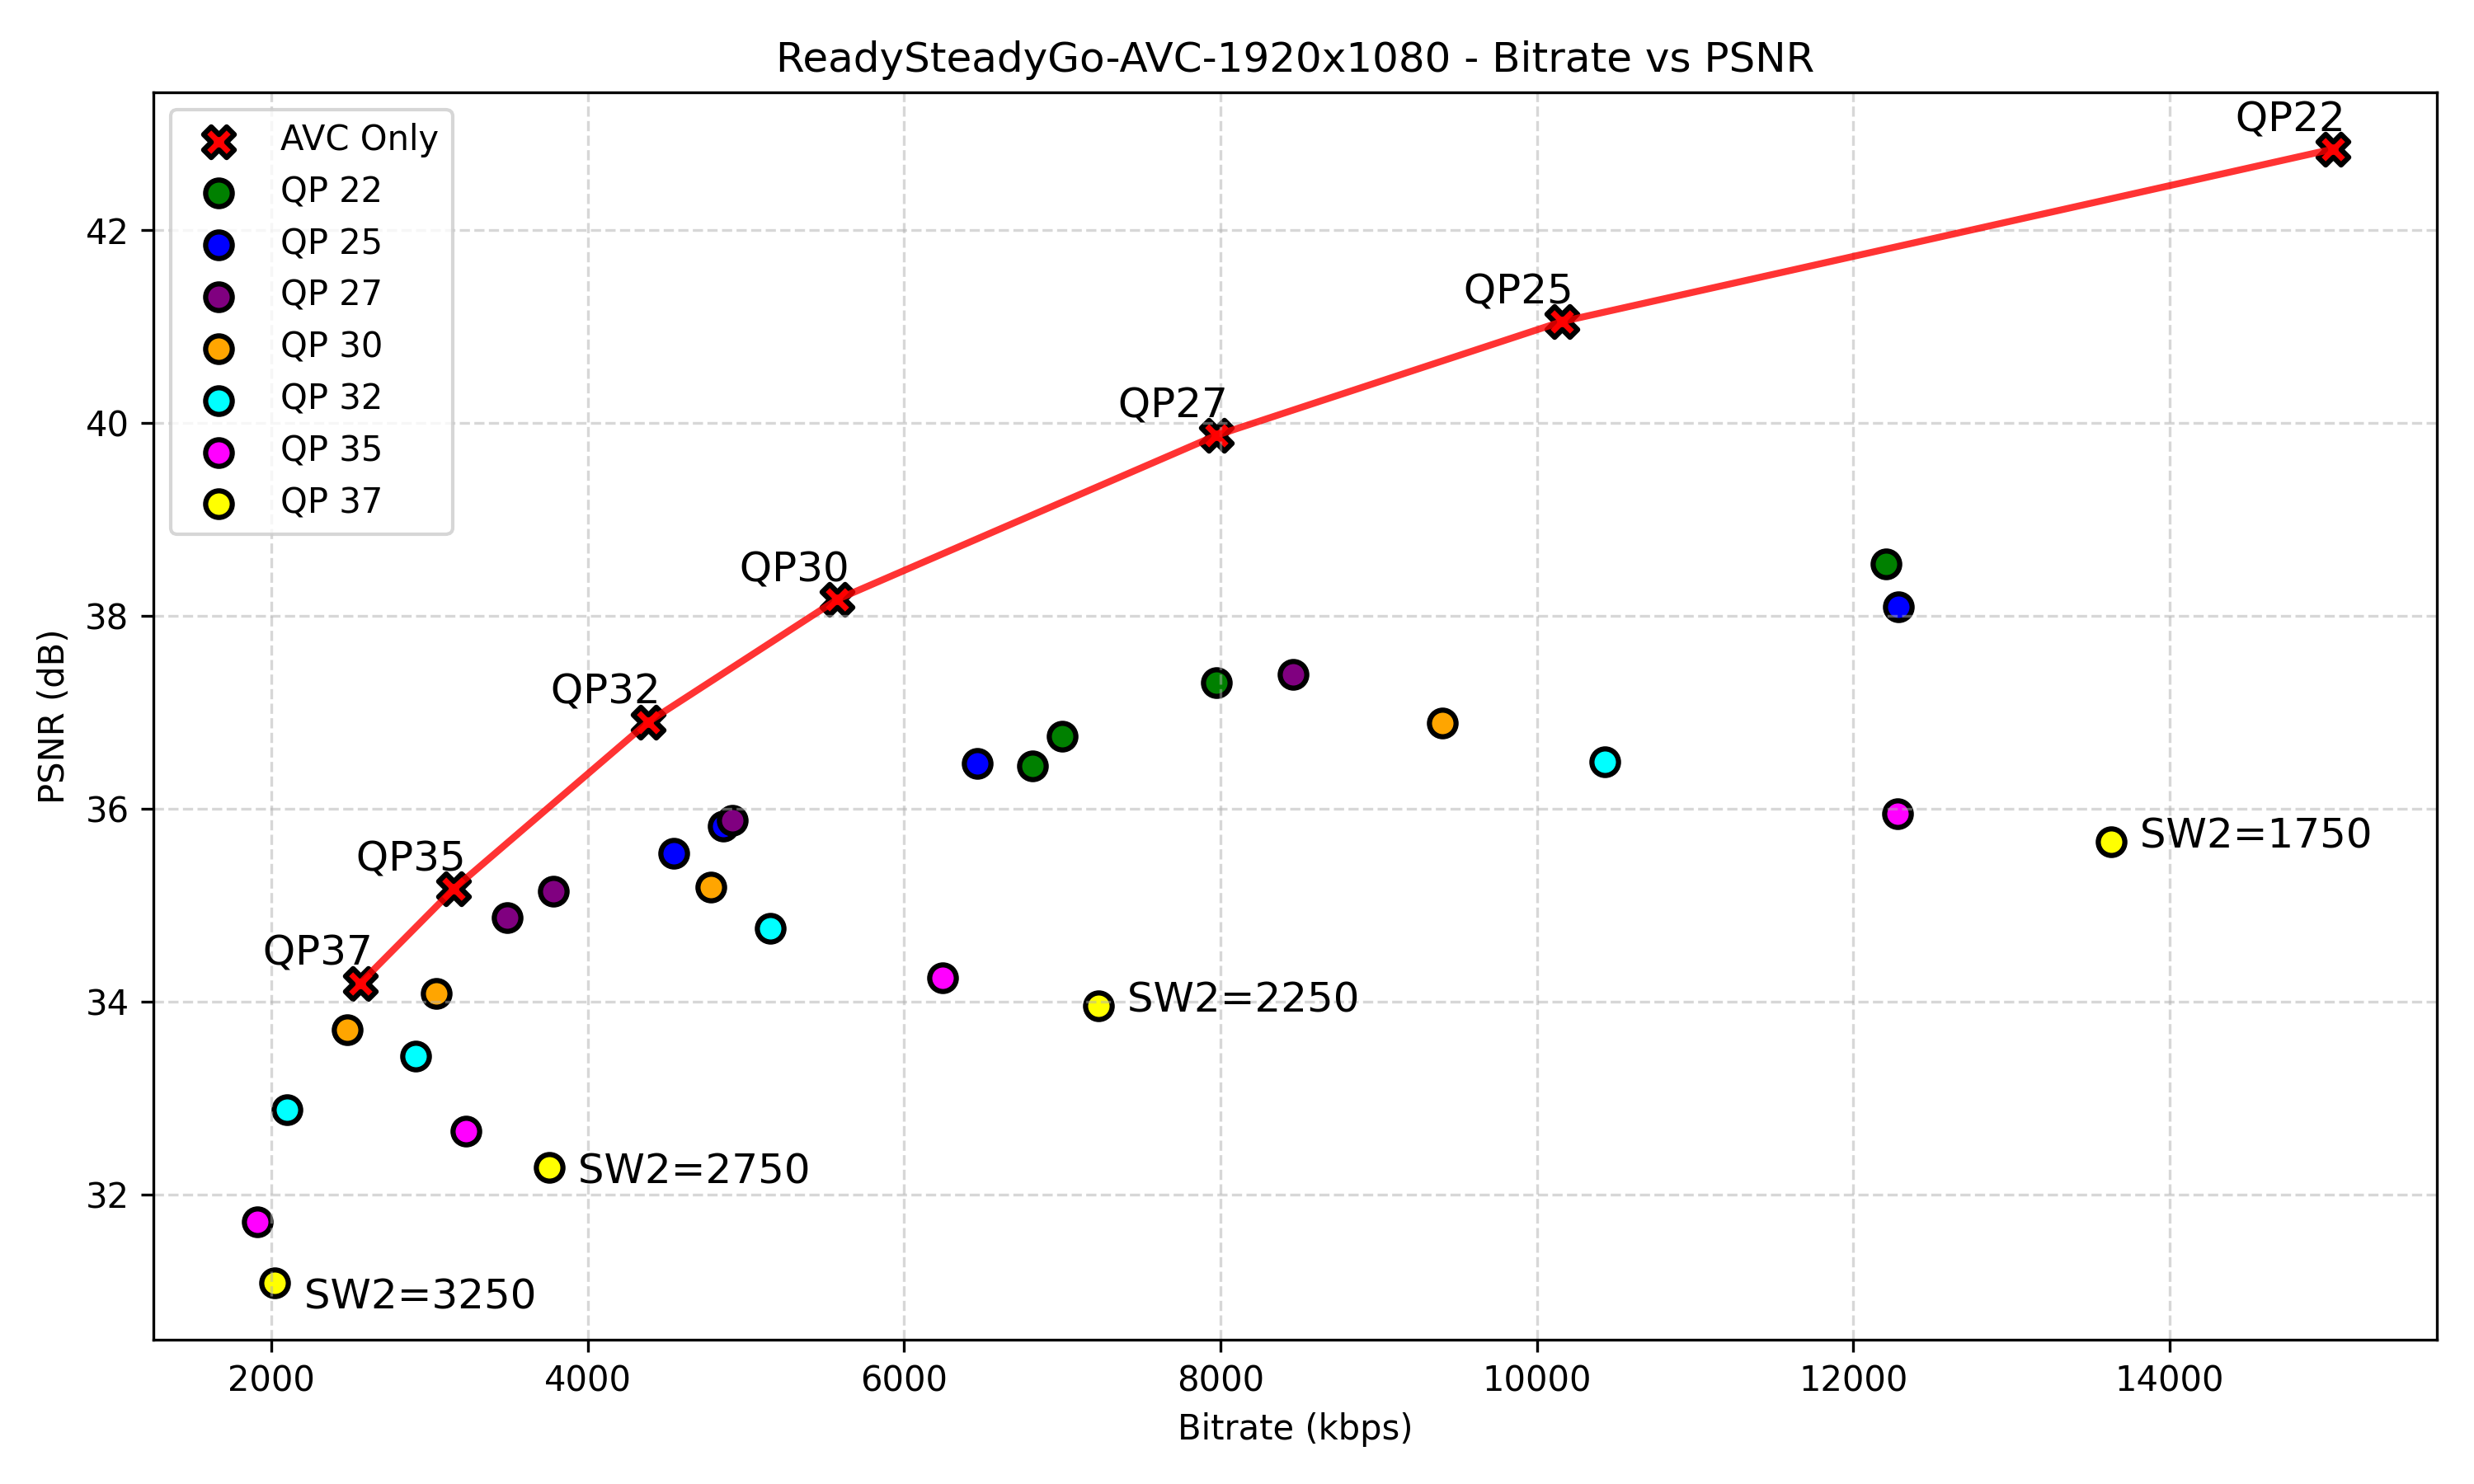
\includegraphics[width=1.0\textwidth]{img/ReadySteadyGo-AVC.png}
    \caption{Resultados para "ReadySteadyGo"\ em \acrshort{AVC}. \cite{uvg_dataset}}
    \label{fig:RSG}
\end{figure}

Em geral, os resultados para esta sequência não demonstraram superioridade clara
em comparação com o \acrshort{AVC} puro.

Nos testes com o SW2 = 1250, os resultados demonstram \textit{bitrates} 
significativamente mais altos, com ganhos pequenos ou mesmo nulos em \acrshort{PSNR}.
Mesmo em configurações com um QP menor, o \acrshort{LCEVC} demonstrou um \textit{bitrate}
muito alto, sem nenhuma melhoria de qualidade.

Para valores intermediários de SW2, houve uma redução no \textit{bitrate}, mas
também houve uma queda no \acrshort{PSNR}.

Em valores maiores de SW2, a camada de aprimoramento passou a ter pouca ou nenhuma
relevância, com taxas abaixo dos 10\%. Com isso, os resultados se aproximam do
desempenho da camada base, com valores baixos de \acrshort{PSNR}, acarretando
em uma perda significativa de qualidade.

Desta forma, esta sequência não se beneficiou com o uso do \acrshort{LCEVC}, onde
a relação entre \acrshort{PSNR} e \textit{bitrate} foi mais favorável ao \acrshort{AVC}
puro.

Vale destacar que o \textit{Resample} do \acrshort{LCEVC} obteve um \acrshort{PSNR}
relativamente baixo em relação aos resultados obtidos. Isto demonstra, que possivelmente,
os resíduos que foram perdidos neste processo, foram compensados pela camada de 
aprimoramento

\newpage
\subsection{Jockey}

\begin{figure}[h!]
    \centering
    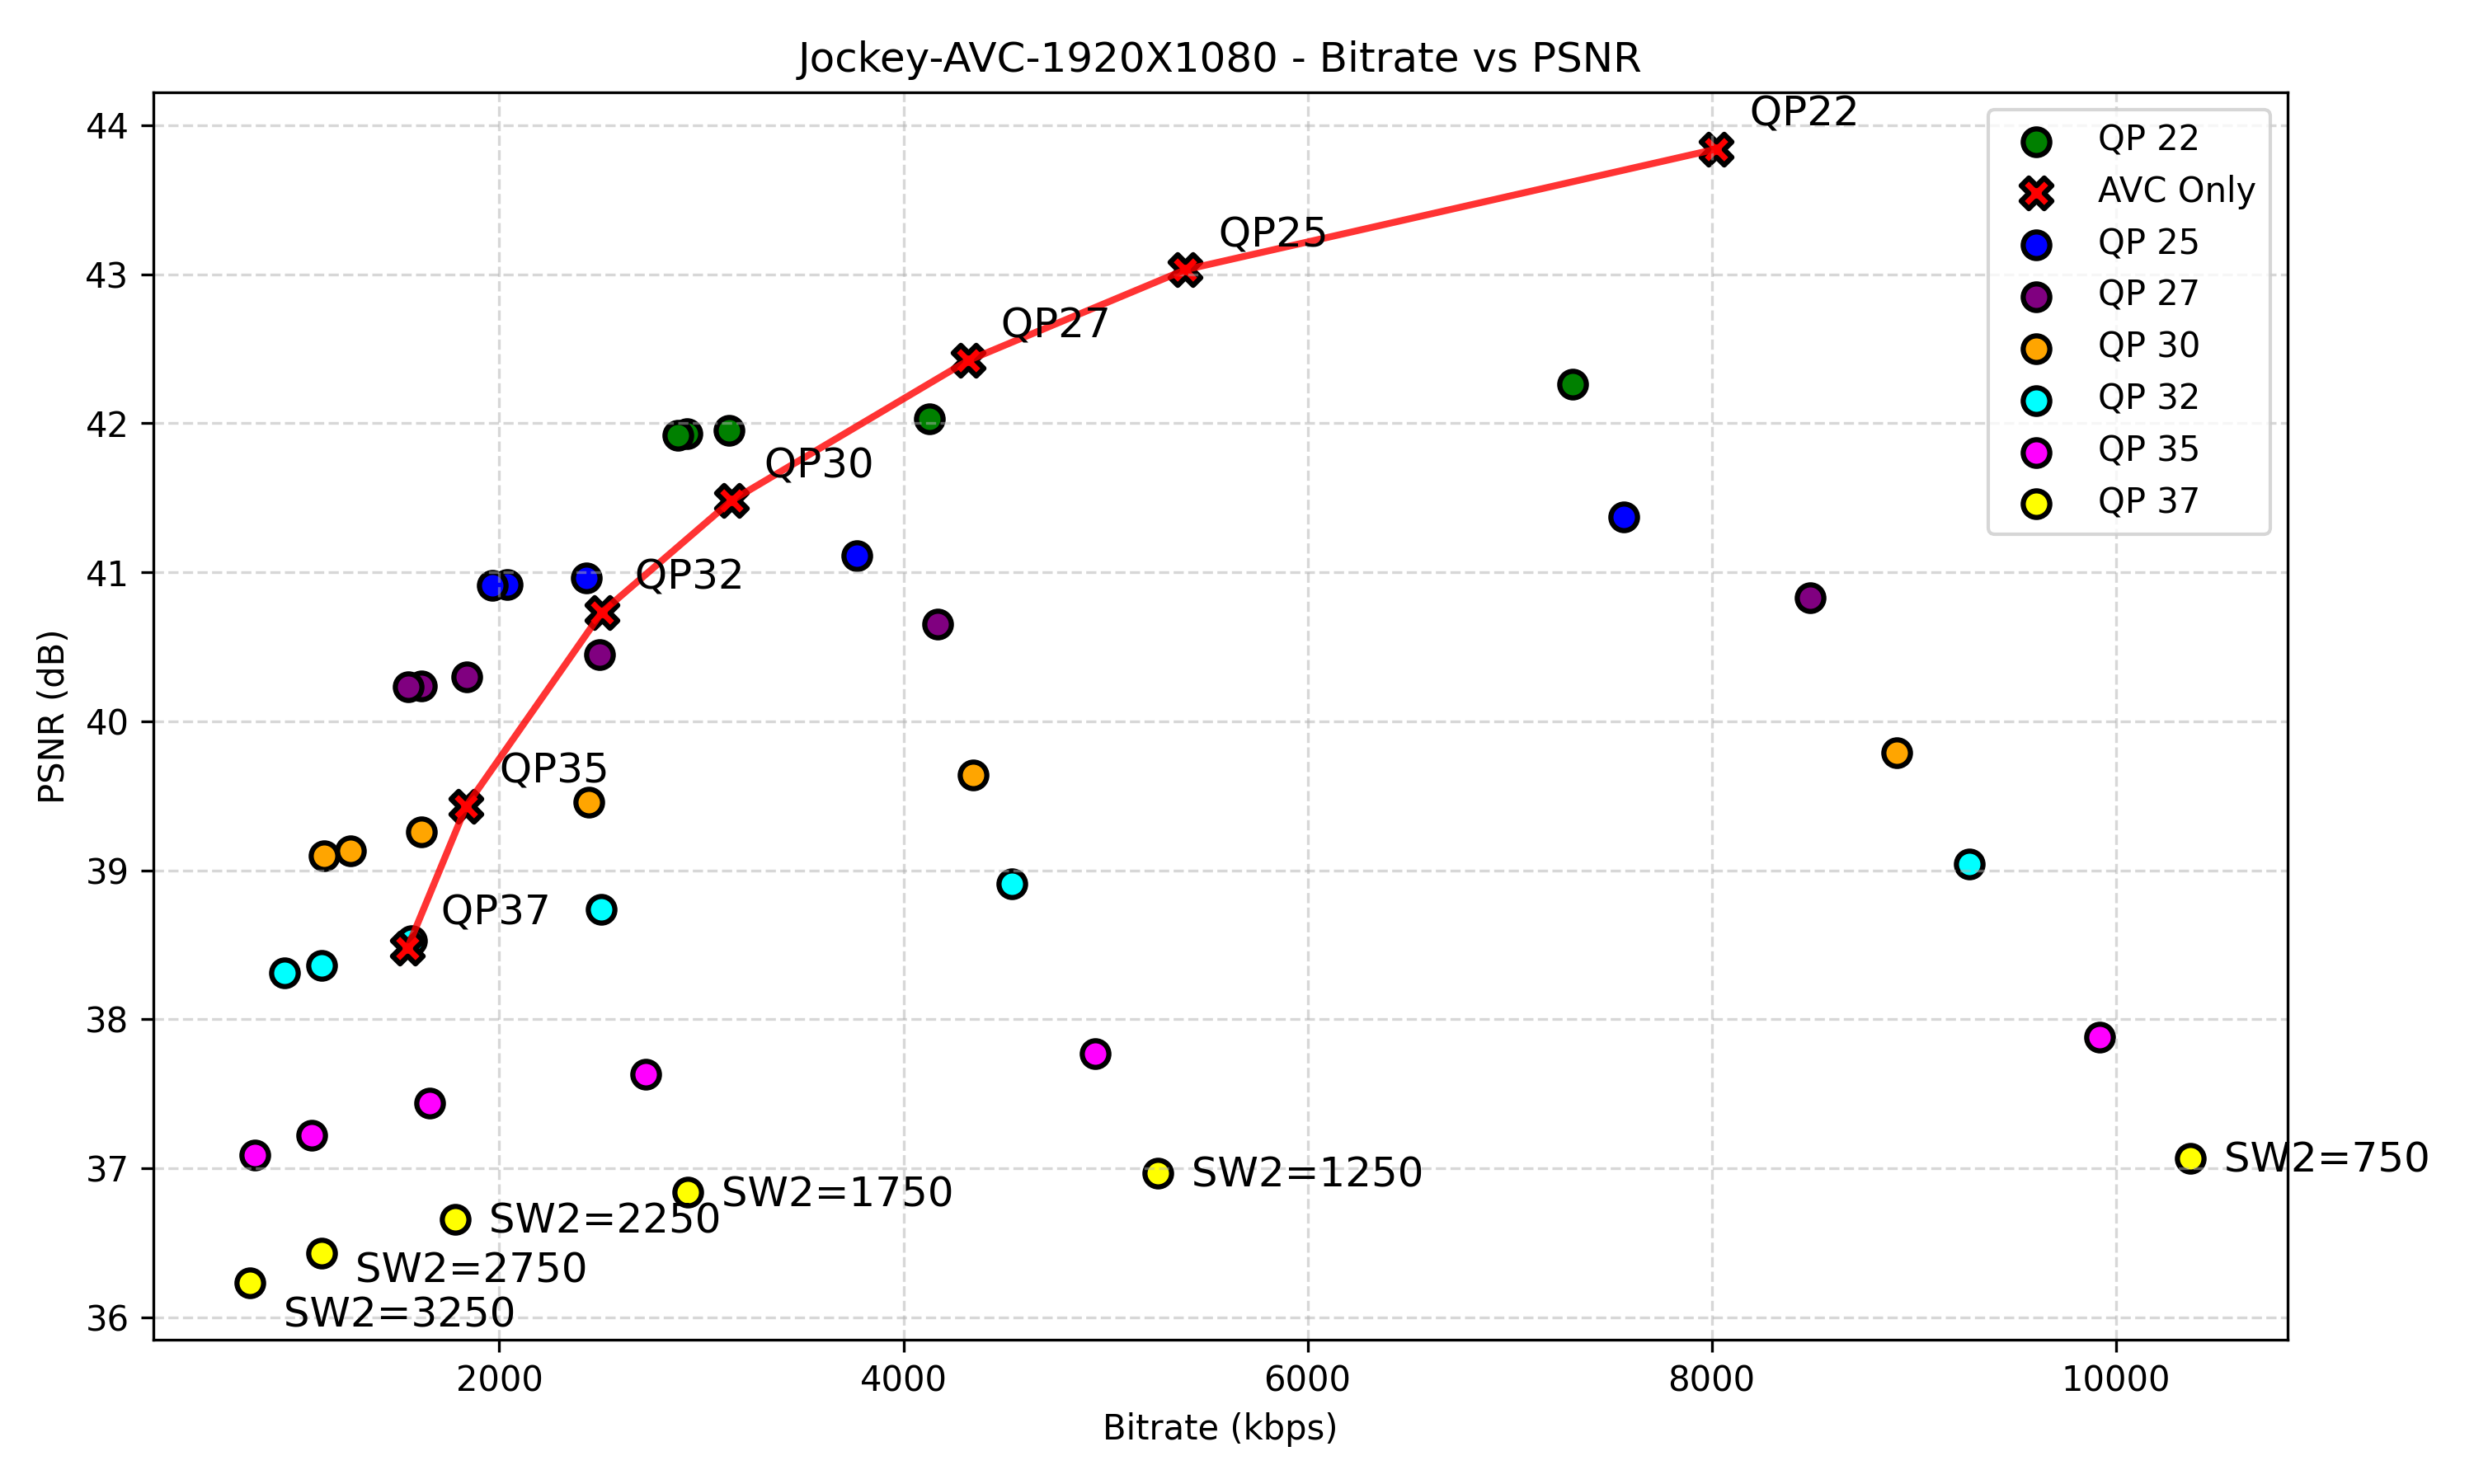
\includegraphics[width=1.0\textwidth]{img/Jockey-AVC.png}
    \caption{Resultados para "Jockey"\ em \acrshort{AVC}. \cite{uvg_dataset}}
    \label{fig:Jockey}
\end{figure}

Para a sequência \textit{Jockey}, o \acrshort{LCEVC} alcançou ótimos resultados
em relação às sequências de referência, onde há casos em que o \acrshort{LCEVC}
demonstrou um \acrshort{PSNR} superior com um \textit{bitrate} menor. Percebe-se
este comportamento em vários pontos antes do QP27 das sequências de referência.
A partir desse ponto, o valores testados para o \acrshort{LCEVC} decaem e não
são mais os melhores valores. Entretanto, considerando os resultados obtidos,
é possível que com mais testes, surjam mais valores em que o \acrshort{LCEVC}
se sai melhor.

Aqui, vemos um caso em que o \acrshort{LCEVC} se destacou e demonstrou vantagens
em comparação ao \acrshort{AVC} exclusivo, especialmente em configurações de 
\textit{bitrate} intermediários.

Em valores mais baixos, o \acrshort{LCEVC} alcançou \acrshort{PSNR} elevados
com \textit{bitrates} competitivos. Apesar do \textit{bitrate} mais alto,
a relação qualidade-tamanho mostra que o \acrshort{LCEVC} pode ser viável
para aplicações que priorizam a qualidade visual.

Na faixa média, o \acrshort{LCEVC} equilibrou melhor eficiência e qualidade,
superando o \acrshort{AVC} puro. 

Para valores mais altos de SW2, a contribuição da camada de aprimoramento
diminuiu, aproximando-se dos valores de somente \acrshort{AVC}, mas ainda
com ganhos moderados de \acrshort{PSNR}.

Dessa maneira, o \acrshort{LCEVC} é particularmente eficaz para conteúdos
dinâmicos como "Jockey", onde a camada de aprimoramento compensa perdas da
compressão base sem aumentas excessivamente o \textit{bitrate}.

\subsection{SOCCER}

\begin{figure}[h]
    \centering
    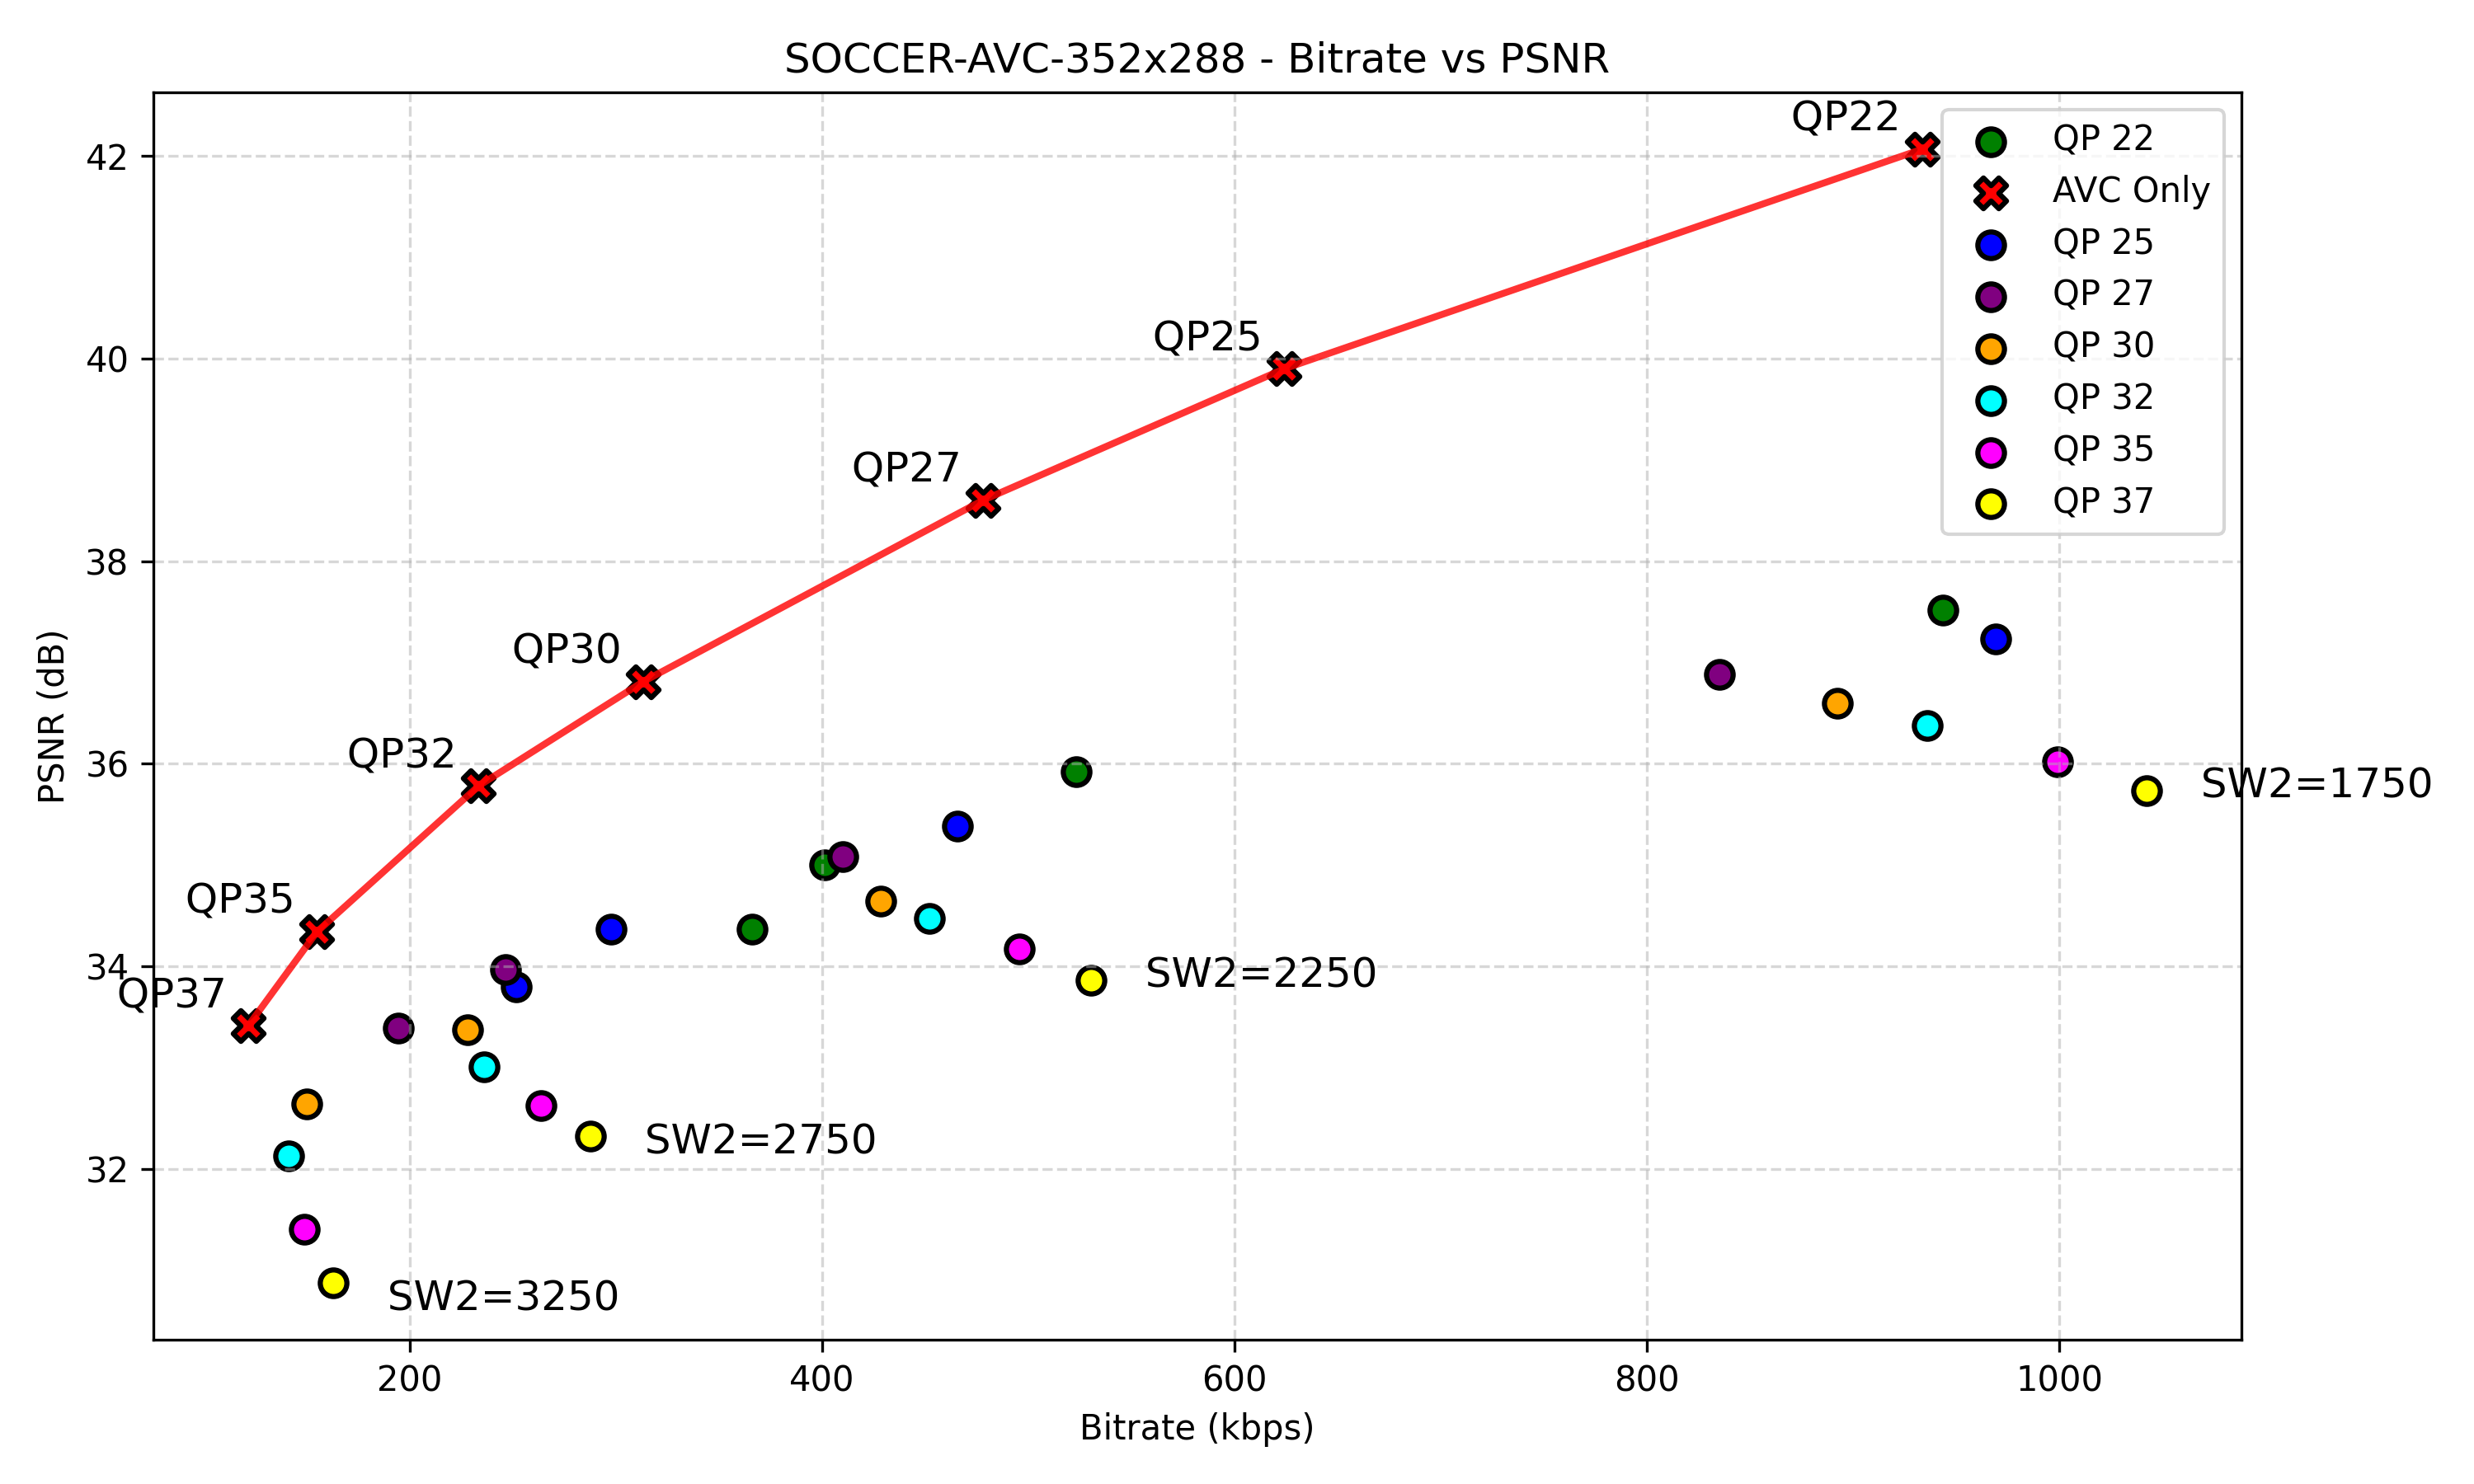
\includegraphics[width=1.0\textwidth]{img/SOCCER-AVC.png}
    \caption{Resultados para "SOCCER"\ em \acrshort{AVC}. \cite{xiph}}
    \label{fig:SOCCER}
\end{figure}

Os resultados indicam que o \acrshort{LCEVC} não apresentou vantagem clara em relação
a somente o \acrshort{AVC} na maioria das configurações testadas.

Em valores mais baixo, o \acrshort{LCEVC} gerou arquivos com \textit{bitrates} altos
para pouco ganho em \acrshort{PSNR}, enquanto o \acrshort{AVC} puro atingiu qualidade
similar com taxas de bits muito menores.

Nas faixas intermediárias de SW2, o \acrshort{LCEVC} reduziu o \textit{bitrate}, mas
com perda acentuada de \acrshort{PSNR}, ficando abaixo da curva de eficiência de somente
o \acrshort{AVC}.

Já em SW2 com valores maiores, a camada de aprimoramento se tornou irrelevante, resultando em
desempenho próximo ao da camada base \acrshort{AVC}, porém ainda inferior ao \acrshort{AVC} puro
em termos de \acrshort{PSNR}.

O \textit{Resample} do \acrshort{LCEVC} também não demonstrou resultados significativos, com 
\acrshort{PSNR} muito abaixo da maioria dos resultados obtidos. 

Assim, o \acrshort{LCEVC} não demonstrou um benefício em ser utilizado nesta sequência.

\newpage
\subsection{City}

\begin{figure}[h]
    \centering
    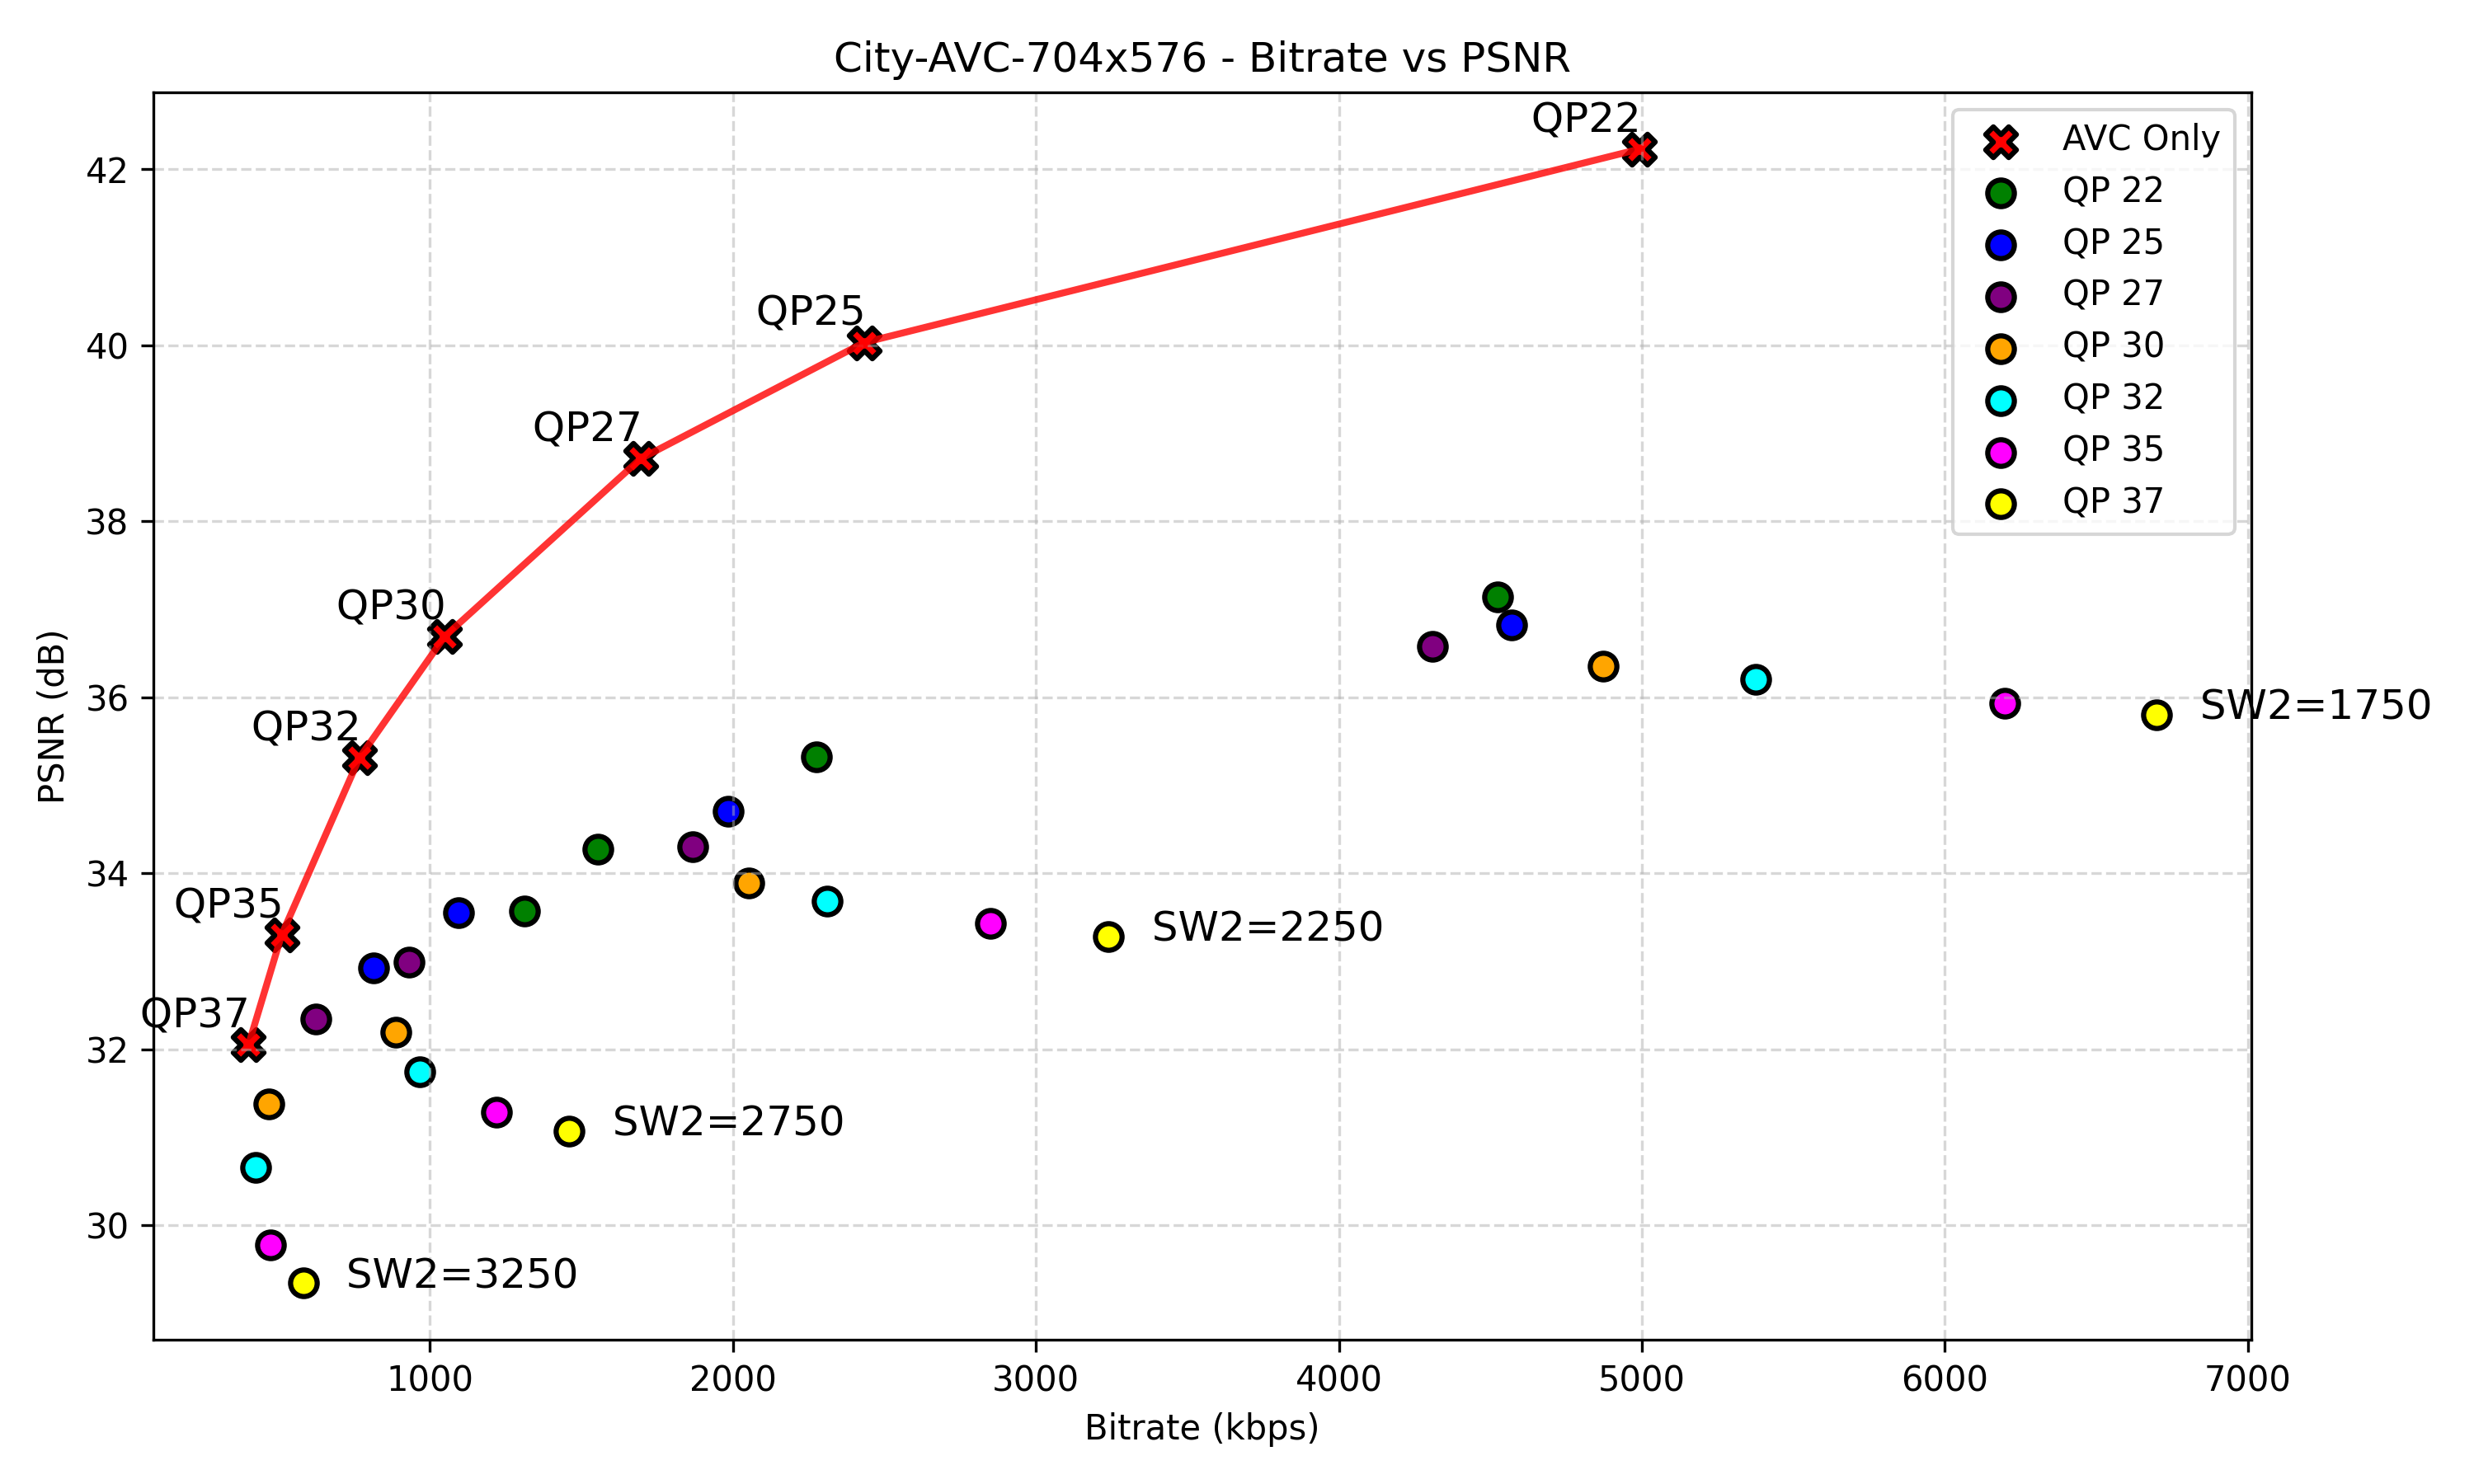
\includegraphics[width=1.0\textwidth]{img/City-AVC.png}
    \caption{Resultados para "City"\ em \acrshort{AVC}. \cite{xiph}}
    \label{fig:City}
\end{figure}

Para esta sequência, os valores intermediários de SW2 proporcionam os resultados mais equilibrados.
Nesses casos, o \acrshort{LCEVC} foi capaz de gerar reconstruções visuais com ganhos notáveis
em qualidade em relação ao \acrshort{AVC}, porém com um ganho notável em \textit{bitrate}.

Percebe-se que para valores iniciais de SW2, que é 250, os valores
obtidos estão aproximadamente na curva que representa os melhores valores, porém, considerando
o valor para \acrshort{AVC} com QP37, ele possui o mesmo \textit{bitrate} de todos os pontos
iniciais do \acrshort{LCEVC}, porém com um \acrshort{PSNR} superior.

Para valores maiores de SW2, o \acrshort{LCEVC} demonstrou um ganho de qualidade, mas foi
um ganho que não acompanhou o ganho em qualidade do \acrshort{AVC} puro, além do aumento
do tamanho da camada de aprimoramento, que acarretou no aumentos do \textit{bitrate}.

O \textit{Resample} do \acrshort{LCEVC} nesta sequência também não demonstrou um resultado
como esperado, ficando com o \acrshort{PSNR} semelhando ao QP35 do \acrshort{AVC} puro,
onde este ponto deveria possui um \acrshort{PSNR} superior aos valores obtidos para o \acrshort{AVC}.

\newpage
\subsection{vc-globo-05}

\begin{figure}[h]
    \centering
    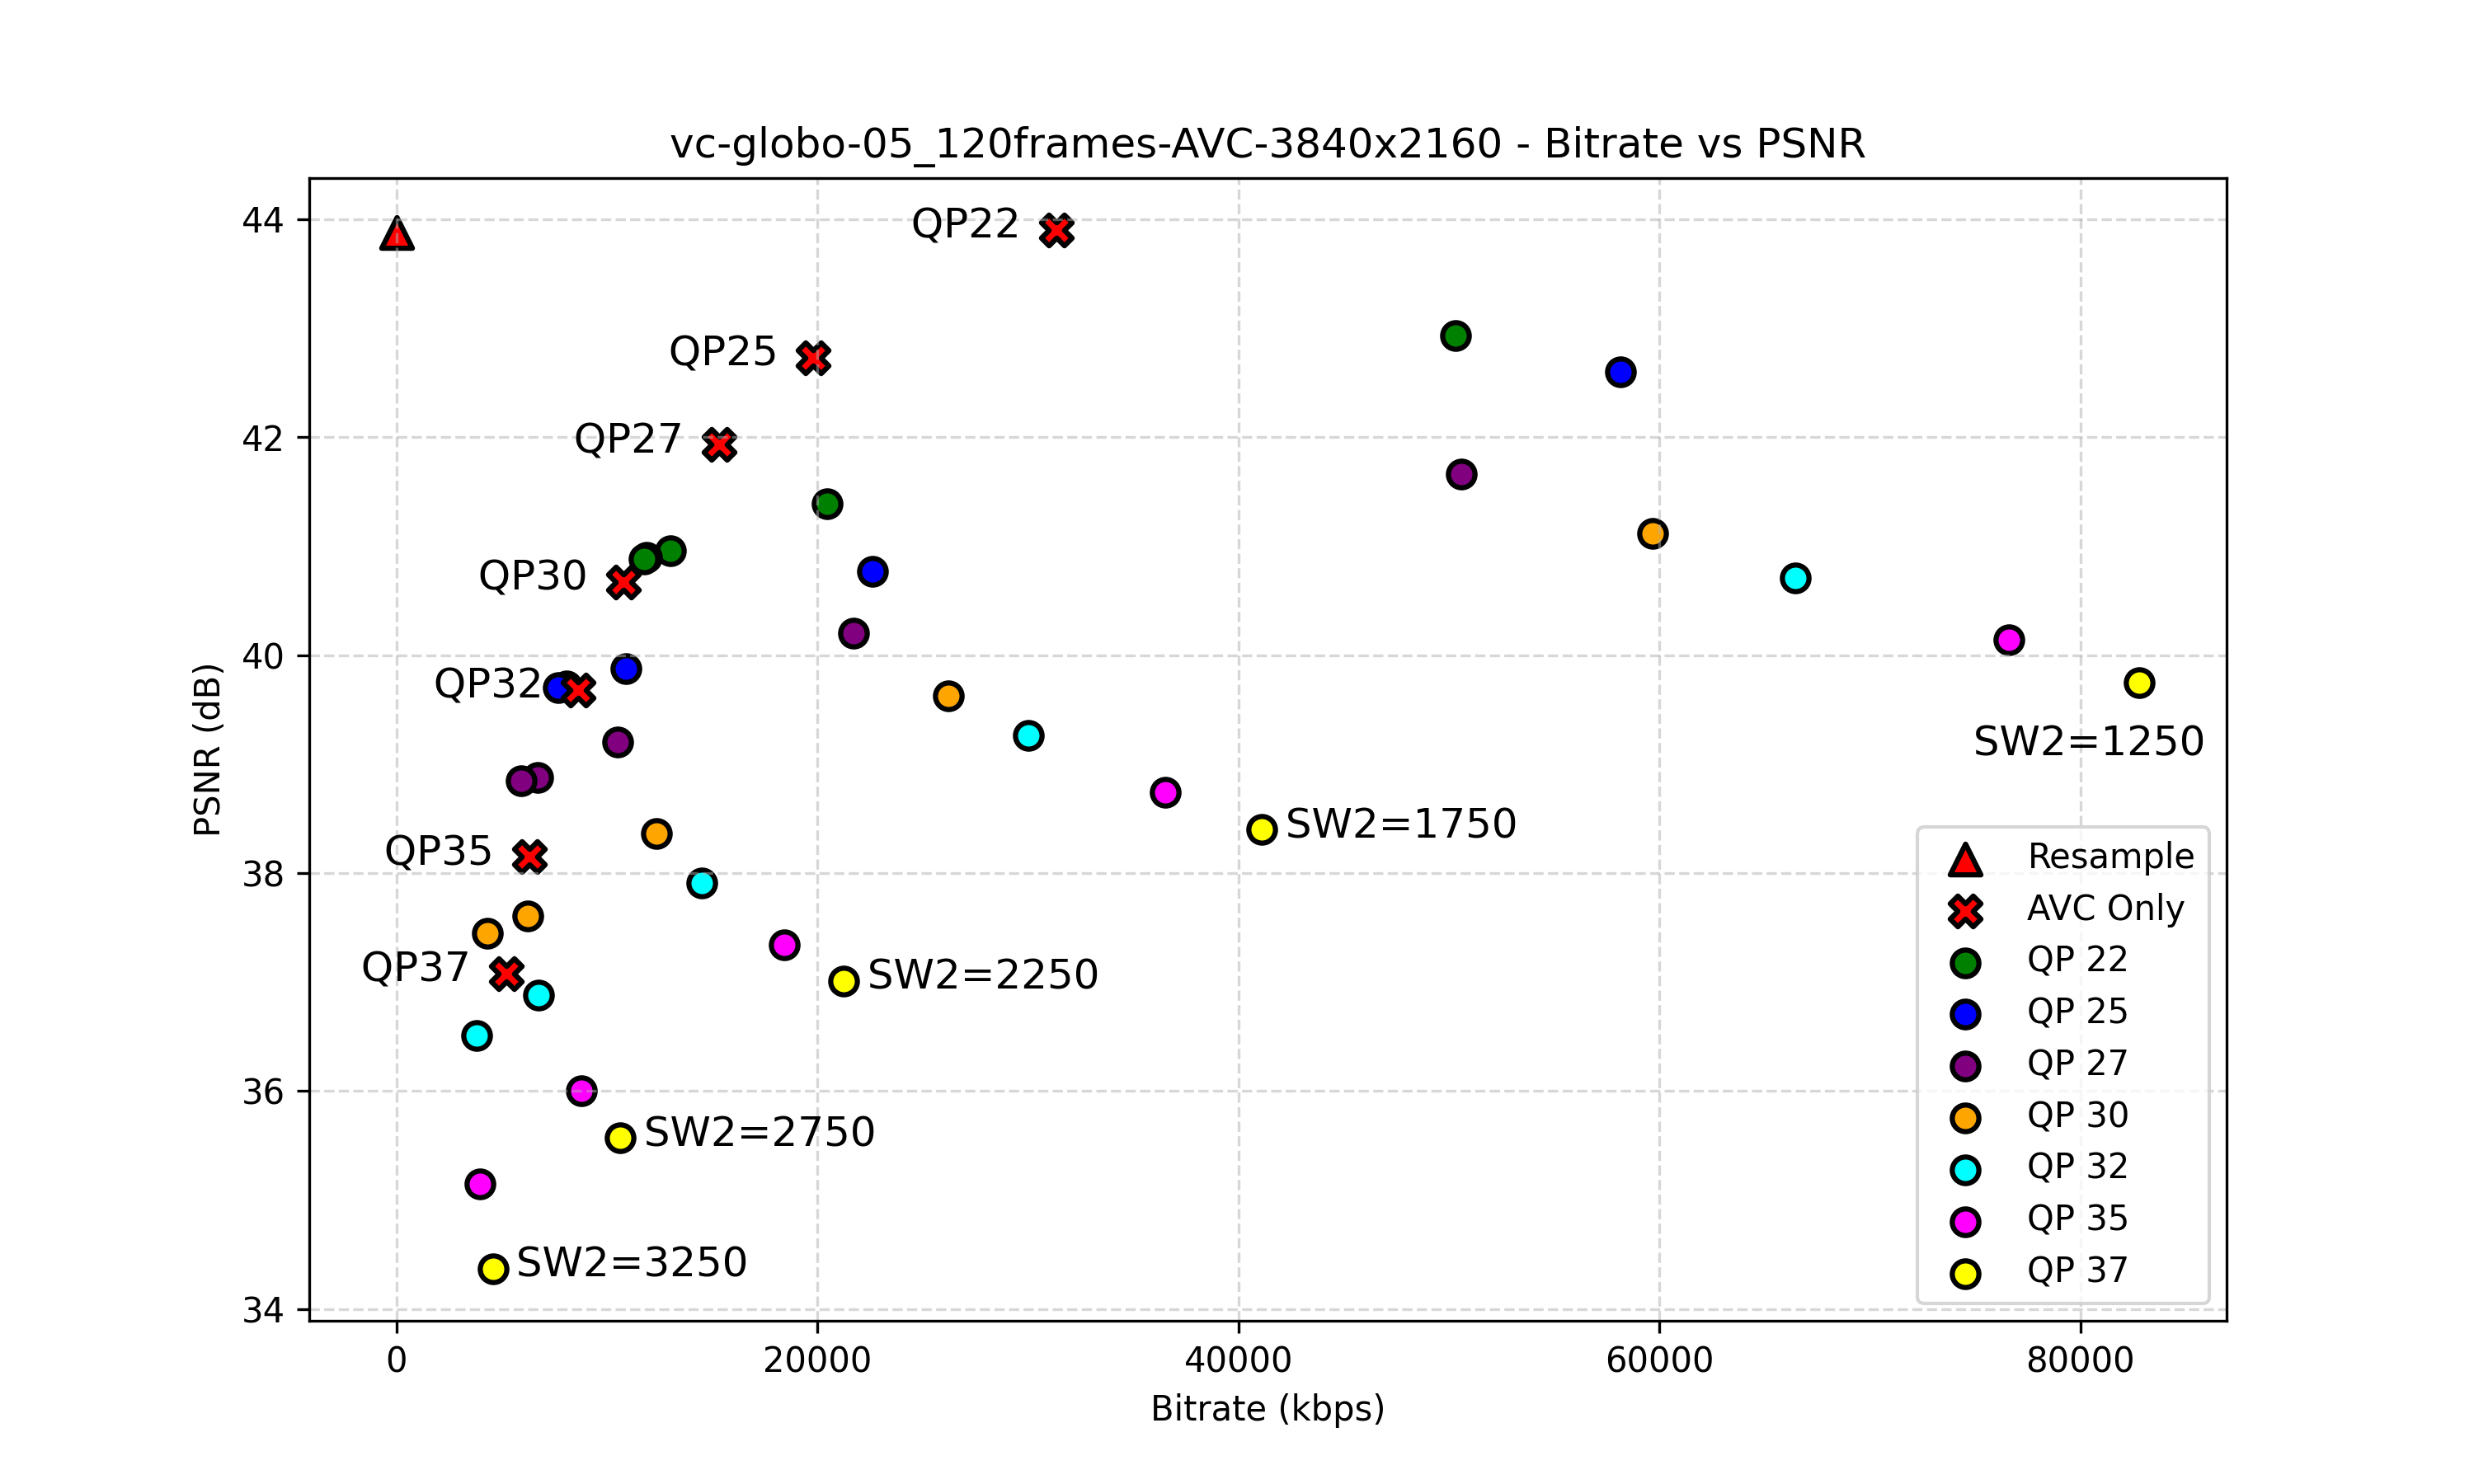
\includegraphics[width=1.0\textwidth]{img/vc-globo-05_120frames-AVC.png}
    \caption{Resultados para "vc-globo-05"\ em \acrshort{AVC}.}
    \label{fig:vc-globo-05}
\end{figure}

Estes resultados mostram que para esta sequência, os resultados obtidos com \acrshort{LCEVC}
foram acima da média em comparação com outros resultados. A curva que resulta dos valores
de SW2 para cada QP com o \acrshort{LCEVC} está mais elevada, demonstrando que houve uma perda
menor de \acrshort{PSNR} e que a qualidade está próxima dos vídeos com somente \acrshort{AVC}.

Para SW2 = 1250, os resultados possuem um \textit{bitrate} bastante elevado em comparação com 
a curva dos vídeos de referência. O que representa que o tamanho do arquivo gerado foi superior
a todos os pontos à esquerda.

Os valores 3250 e 2750 de SW2 resultaram em valores de \acrshort{PSNR} que estão acima da curva
dos vídeos de referência, mostrando que o \acrshort{LCEVC} conseguiu gerar resultados mais
eficientes do que os vídeos que usaram somente o \acrshort{AVC}.

Outro ponto a se observar é que o \textit{Resample} do \acrshort{LCEVC} obteve um valor de 
\acrshort{PSNR} bastante próximo ao valor obtido pelo QP = 22 do \acrshort{AVC}.


\newpage

\subsection{vc-lcevc-01}

\begin{figure}[h]
    \centering
    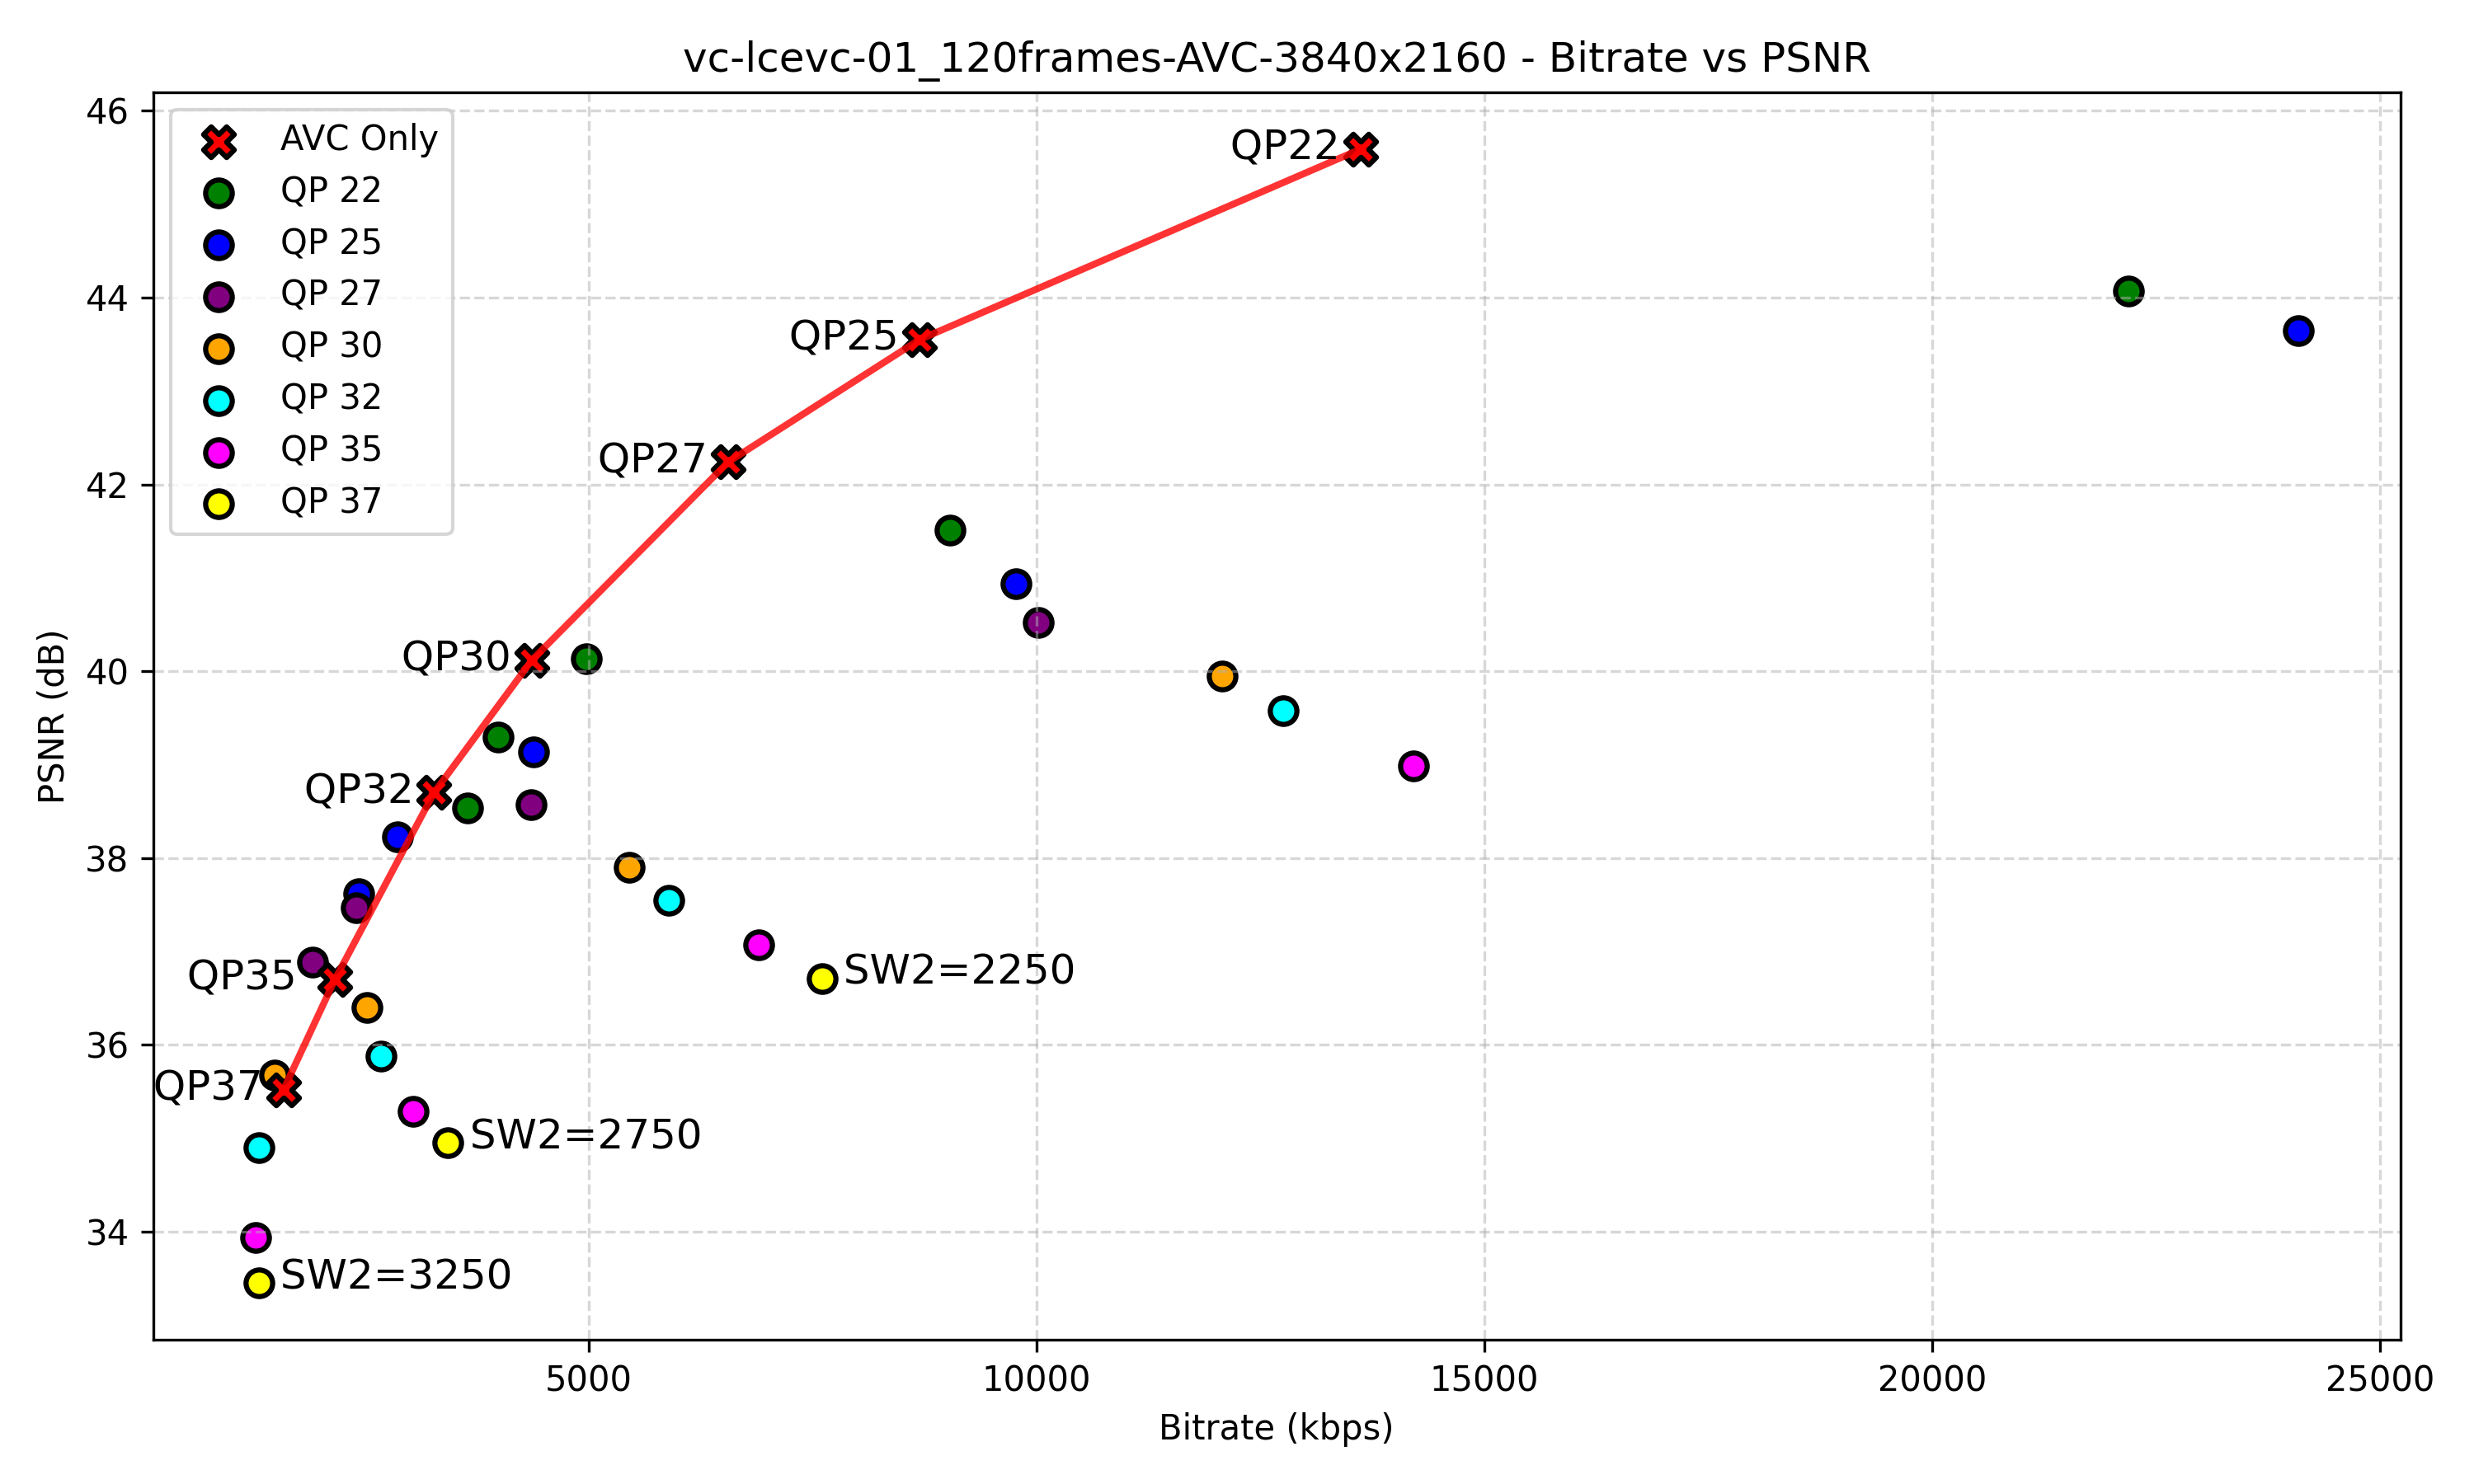
\includegraphics[width=1.0\textwidth]{img/vc-lcevc-01_120frames-AVC.png}
    \caption{Resultados para "vc-lcevc-01"\ em \acrshort{AVC}.}
    \label{fig:vc-lcevc-01}
\end{figure}

Aqui, com o SW2 = 1250, os dados mostraram que a camada de aprimoramento foi fortemente
utilizada, com uma proporção de aprimoramento superior a 90\% em todos os casos, resultando
em um \textit{bitrate} elevado. Reduzindo para o valor 1750, houve uma melhora na eficiência.

Nos valores para SW2 iguais a 1750 e 2250, os resultados foram se aproximando da curva dos
vídeos referência.

Agora, para SW2 com valores de 2750 e 3250, houve uma redução no valor do \textit{bitrate}.
Nestes valores, os resultados foram próximos e até superior aos valores de \acrshort{PSNR}
dos vídeos somente em \acrshort{AVC}.

\newpage

\subsection{vc-philips-01}

\begin{figure}[h]
    \centering
    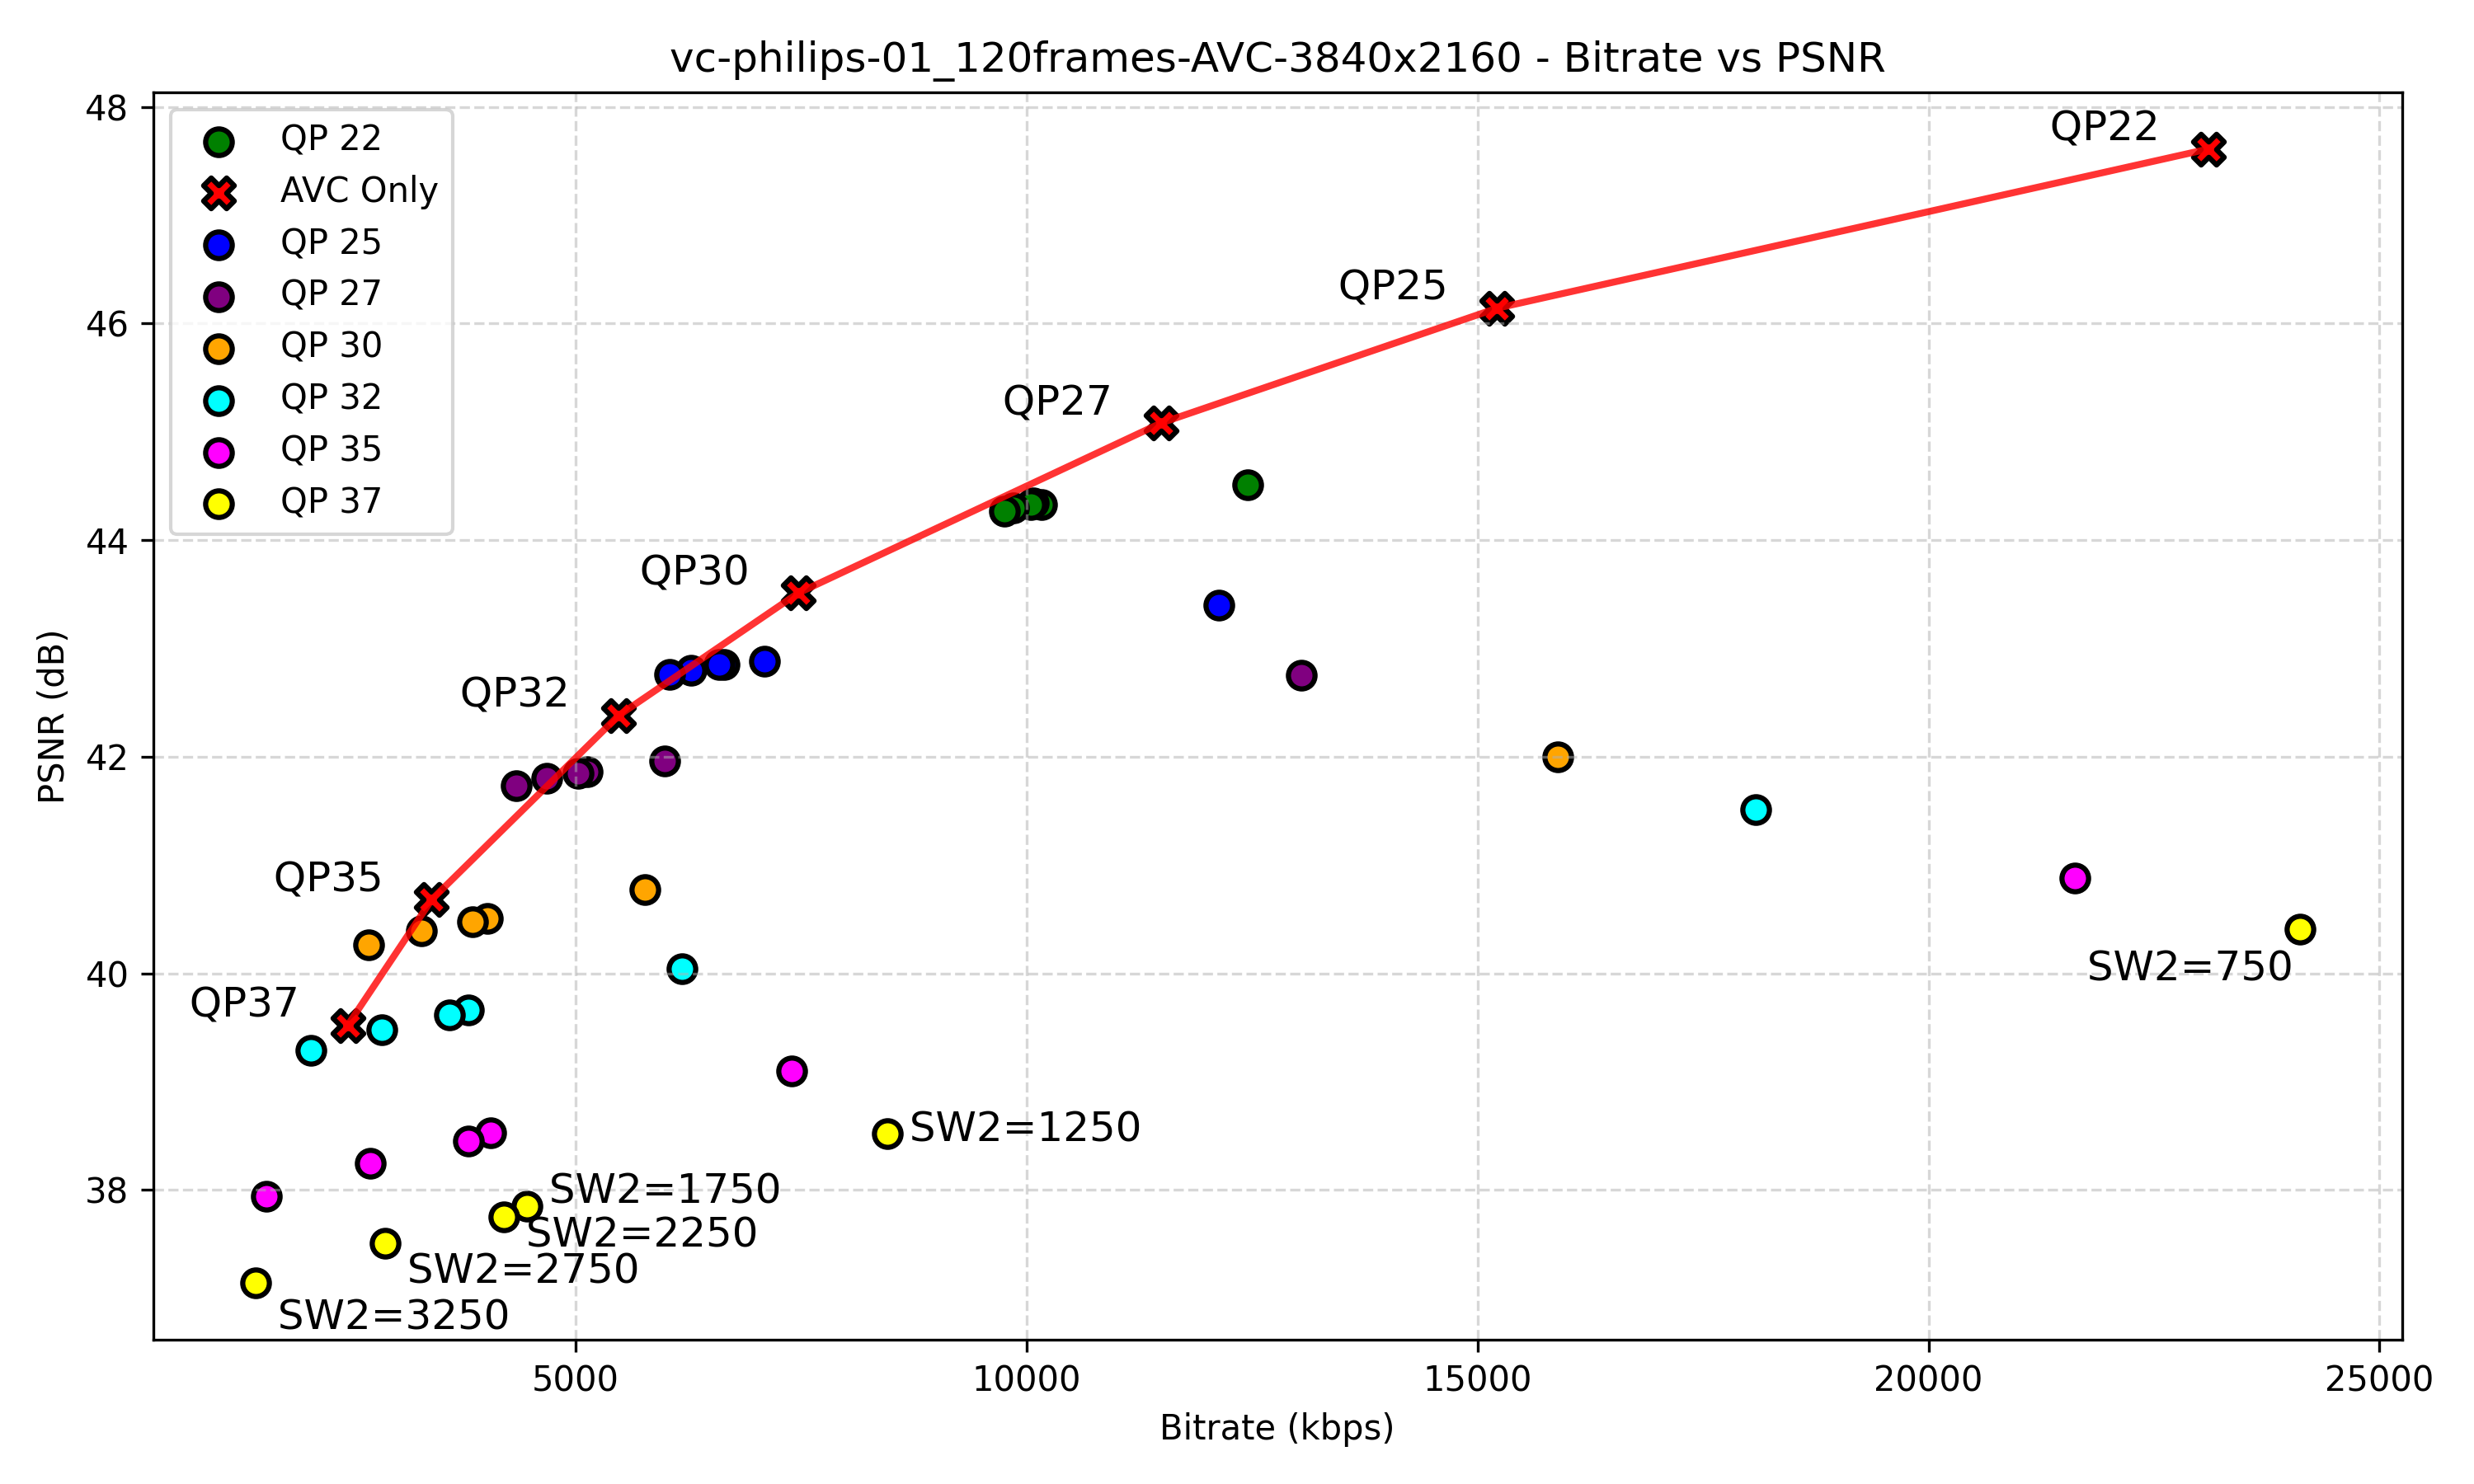
\includegraphics[width=1.0\textwidth]{img/vc-philips-01_120frames-AVC.png}
    \caption{Resultados para "vc-philips-01"\ em \acrshort{AVC}.}
    \label{fig:vc-philips-01}
\end{figure}

A sequência "vc-philips-01" apresentou uma característica interessante: mesmo
com QPs elevados, os valores de \acrshort{PSNR} se mantiveram altos, indicando
que o conteúdo possui um baixo nível de ruído e variação espacial, o que
favorece a compressão.

Nos testes com SW2 = 750, a proporção da camada de aprimoramento variou entre
84\% e 97\%. Para QP = 30, o \acrshort{LCEVC} atingiu 42,00 db a 15,9 Mbps,
enquanto o \acrshort{AVC} alcançou 43,51 db com apenas 7,5 Mbps. Para valores 
como 1250 e 1750 para o SW2, o \textit{bitrate} reduziu drasticamente
para a maioria dos QPs, mantendo o \acrshort{PSNR} alto.

Esta sequência foi bastante interessante, pois para valores de QPs iguais
a 27, 25 e 22 para o \acrshort{LCEVC}, os resultados foram eficientes,
com um \textit{bitrate} semelhante ao do \acrshort{AVC}, onde o \acrshort{LCEVC}
consegue demonstrar superioridade em alguns casos. 

\newpage

\subsection{vc-philips-03}

\begin{figure}[h]
    \centering
    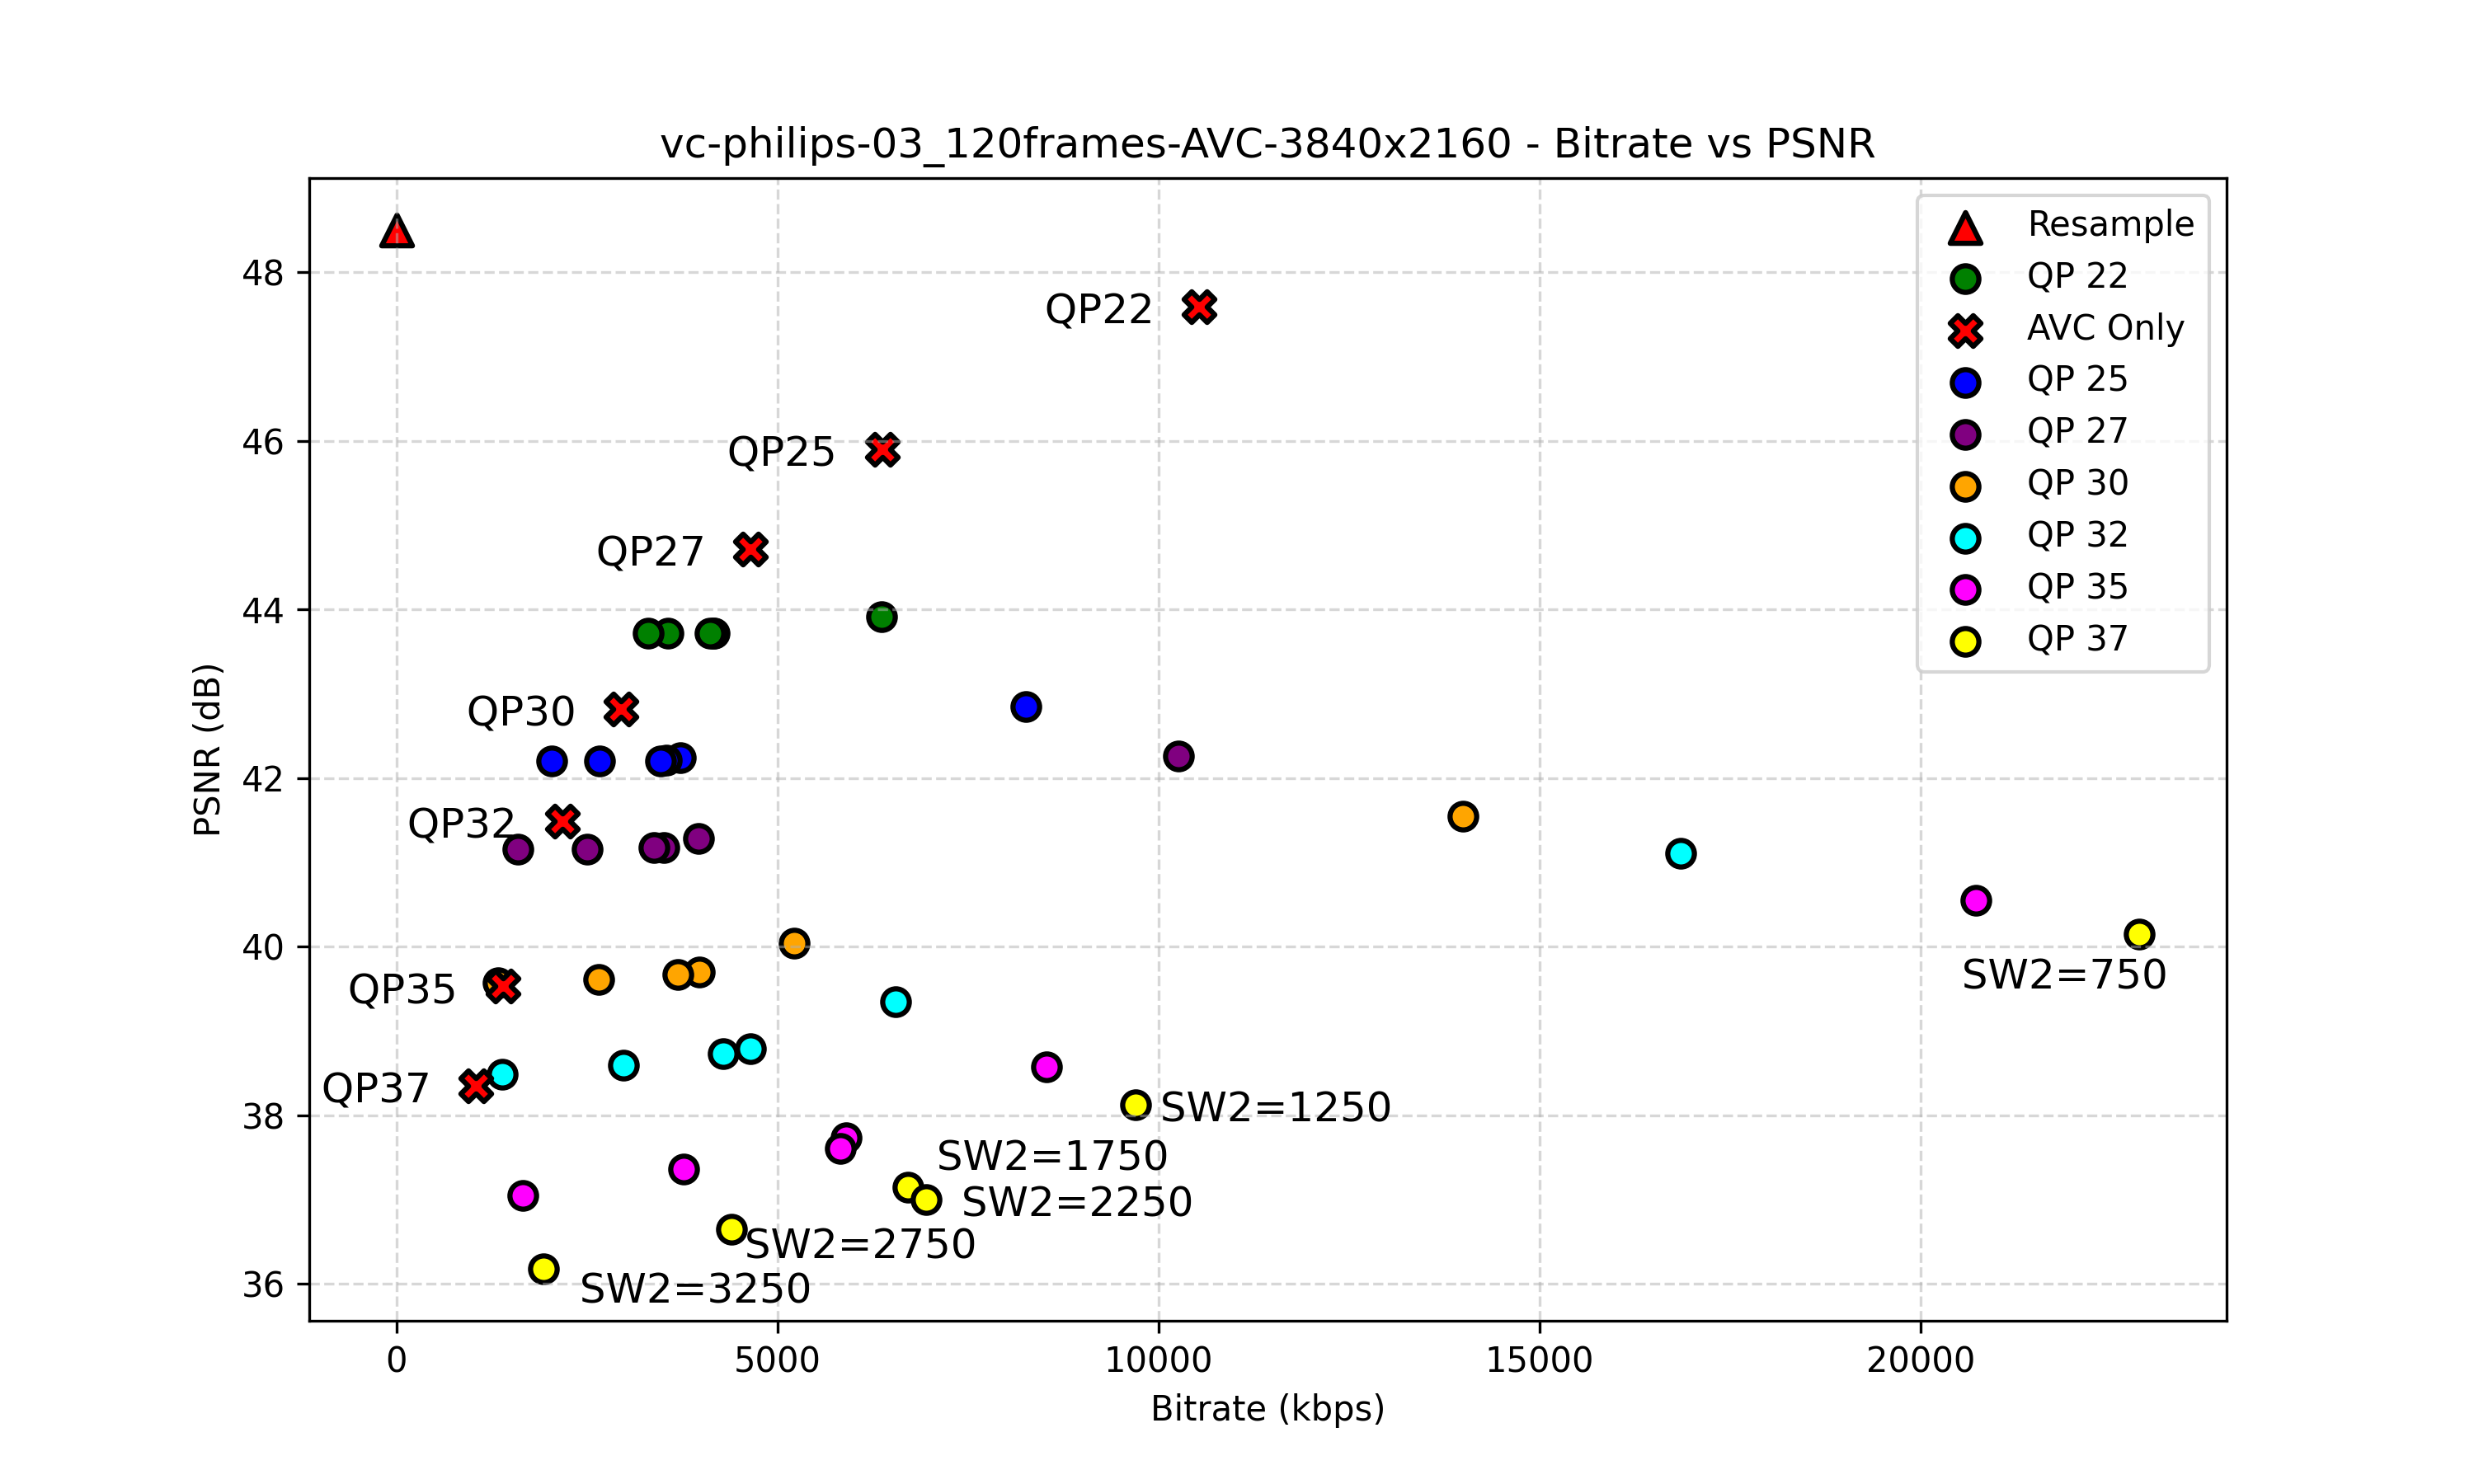
\includegraphics[width=1.0\textwidth]{img/vc-philips-03_120frames-AVC.png}
    \caption{Resultados para "vc-philips-03" em \acrshort{AVC}.}
    \label{fig:vc-philips-03}
\end{figure}

Os resultados obtidos para esta sequência demonstraram um cenário promissor para
o uso do \acrshort{LCEVC}. Com alguns casos em que ele superou o \acrshort{AVC} puro.
Houve um grande aumento do \textit{bitrate} para os resultados entre os valores de SW2
750 e 1250, onde o aumento foi proporcional ao valor do QP da base.

Vale destacar um dos resultados obtidos pela configuração de SW2 = 1250 e QP = 22, onde
o \acrshort{LCEVC} alcançou um \acrshort{PSNR} de 43,72 db com um \textit{bitrate} 
de apenas 4,1 Mbps, enquanto o \acrshort{AVC} alcançou 47,59 db a 10,5 Mbps. Mesmo
com o \acrshort{PSNR} do \acrshort{AVC} sendo superior, a diferença de quase 2,5 vezes
no \textit{bitrate} pode justificar o uso do \acrshort{LCEVC} em cenários com limitação
de banda.

Em posições intermediárias de SW2, como 1750 e 2250, o \textit{bitrate}, o \acrshort{LCEVC}
se aproximou da curva de eficiência do \acrshort{AVC}, para QPs mais baixos, onde para o QP = 22,
por exemplo, esteve bem próximo do \textit{bitrate} do \acrshort{AVC}.

Para o SW2 = 750, o \textit{bitrate} foi muito alto, onde a camada de aprimoramento
consumiu boa parte do tamanho do arquivo, acarretando em um \textit{bitrate} elevado para um
\acrshort{PSNR} relativamente baixo, que não escalou bem com o aumento do QP.

\newpage

\section{VVC}

\subsection{Bosphorus}

\begin{figure}[h]
    \centering
    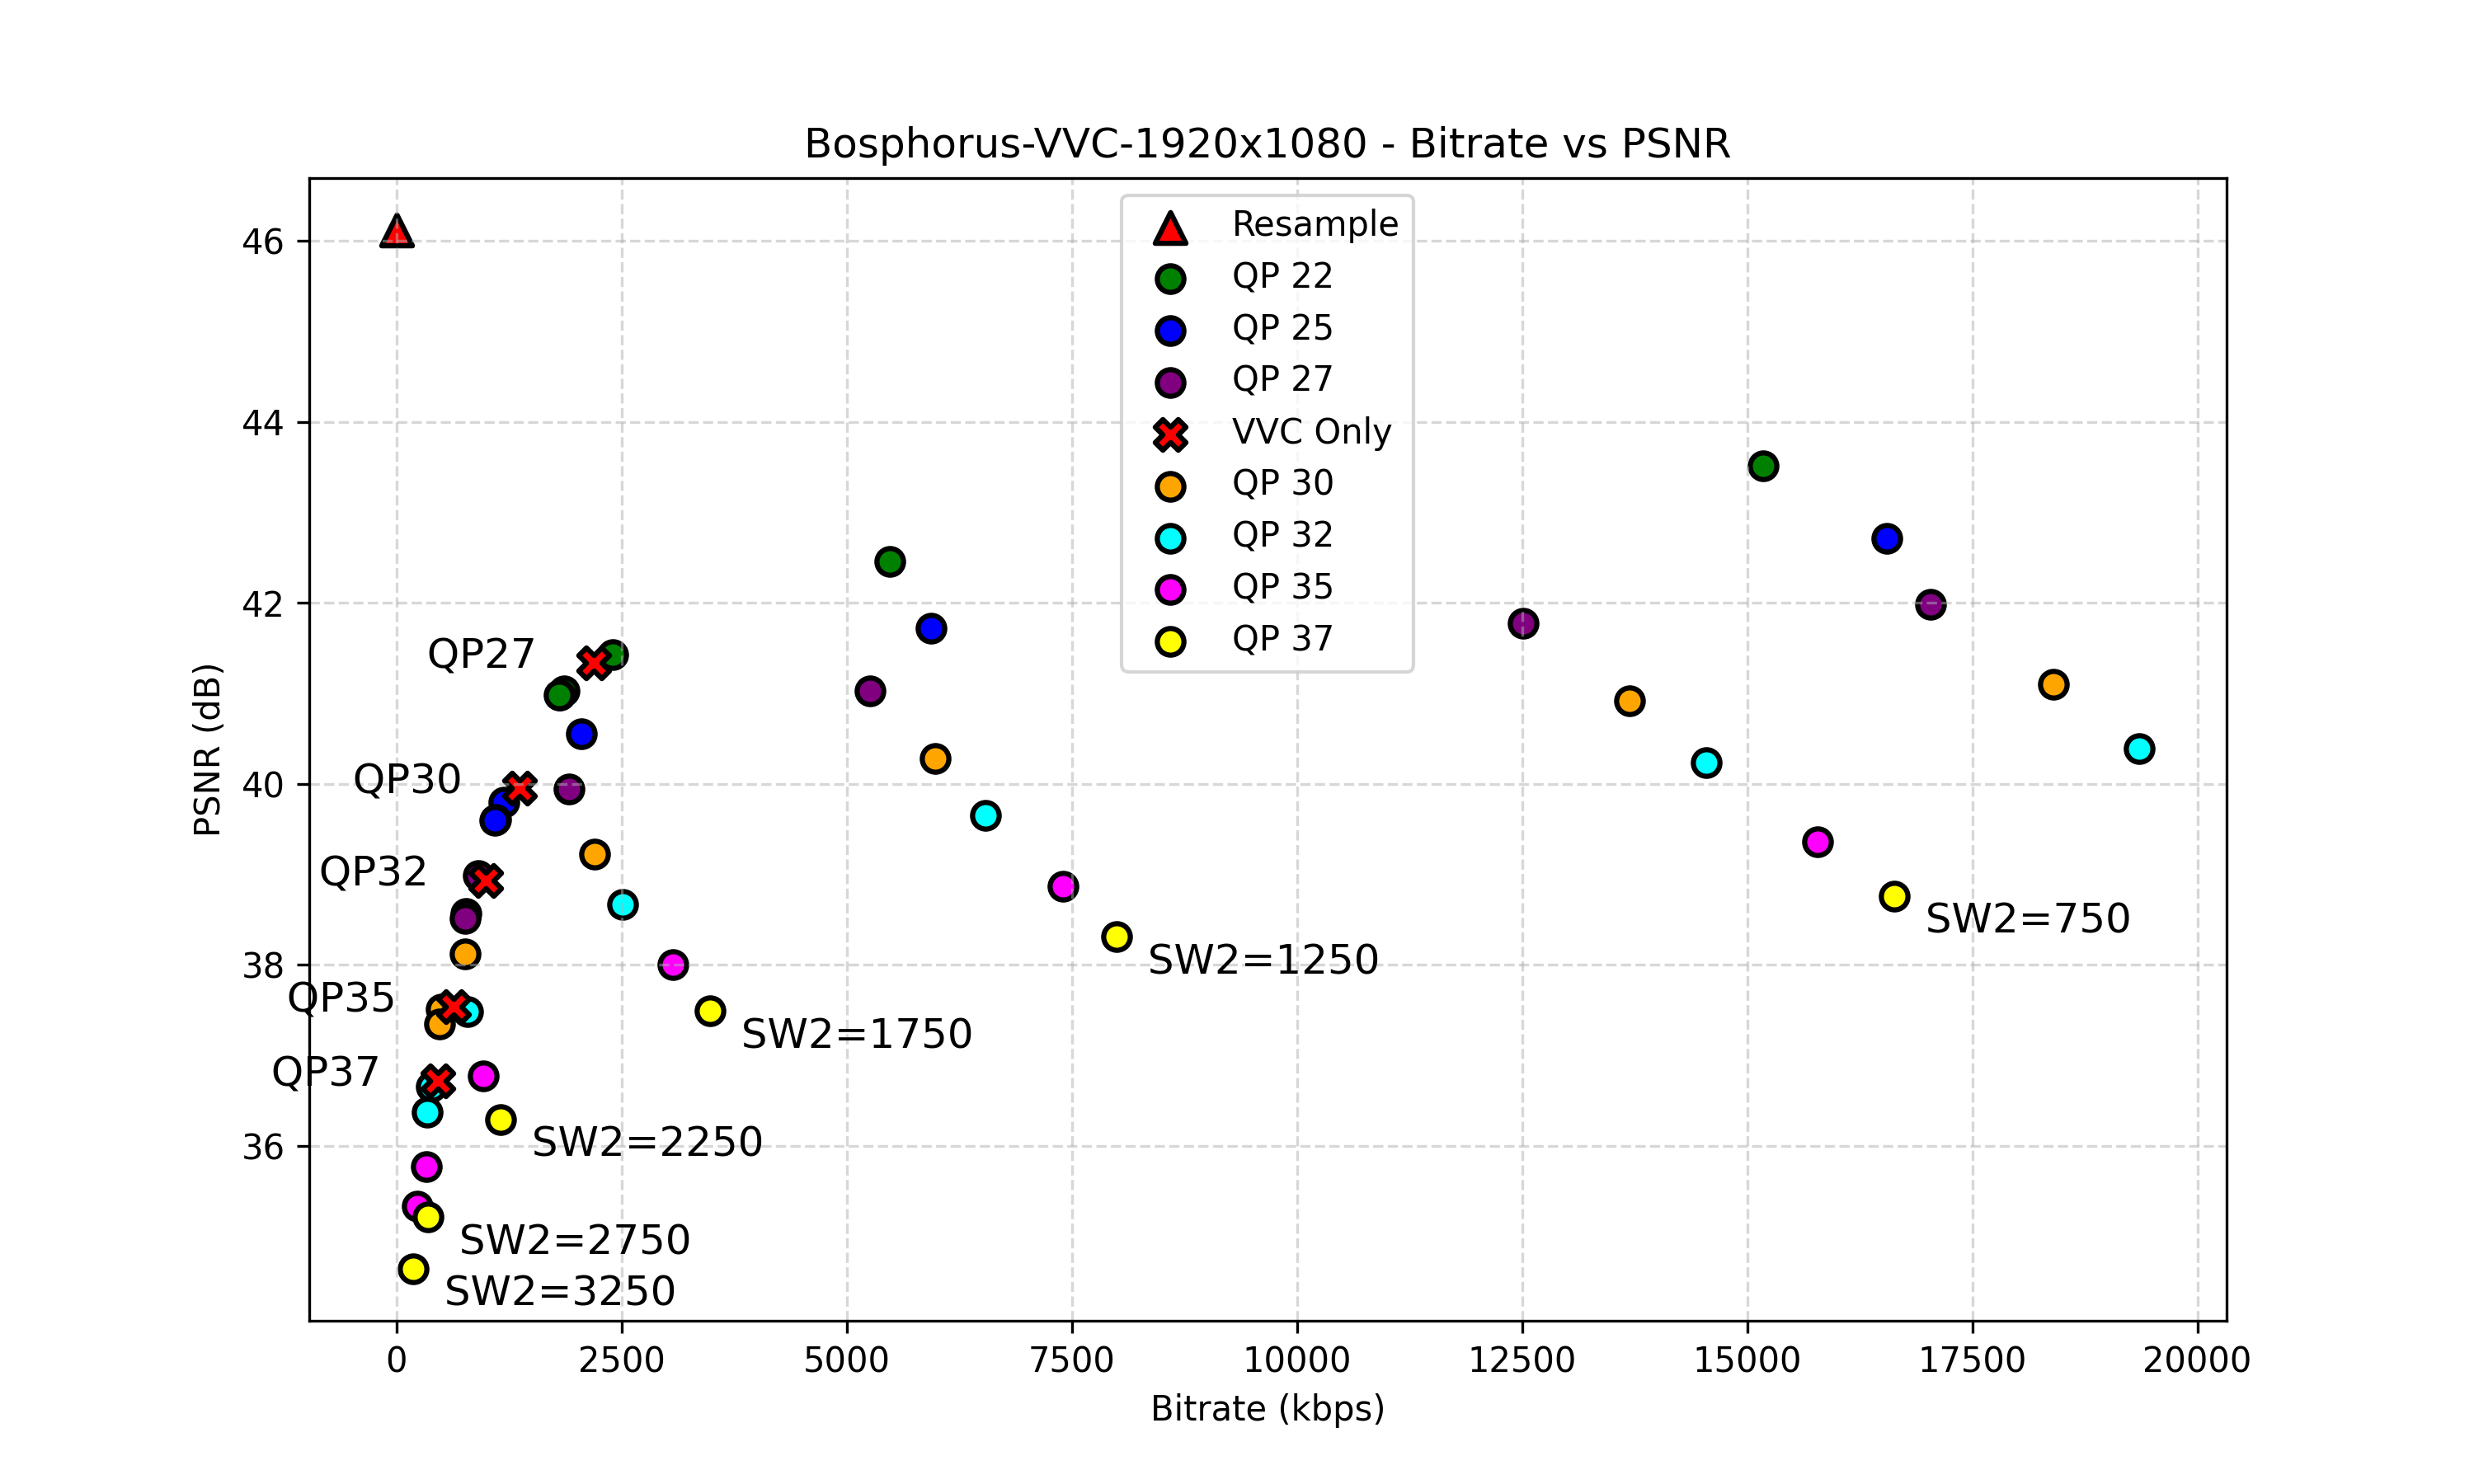
\includegraphics[width=1.0\textwidth]{img/Bosphorus-VVC.png}
    \caption{Resultados para "Bosphorus"\ em \acrshort{VVC}. \cite{uvg_dataset}}
    \label{fig:Bosphorus-VVC}
\end{figure}

Com valores baixos de SW2, a camada de aprimoramento possui peso expressivo no tamanho final
do arquivo, acarretando em um \textit{bitrate} elevado. Embora o ganho de qualidade seja pequeno, 
o aumento de \textit{bitrate} é significativo, tornando estes resultados poucos eficientes.

Para valores intermediários, os valores começam a ter um equilíbrio melhor, se aproximando dos
valores de somente \acrshort{VVC}.

Agora, para valores de SW2 altos, como 3250 e 2750, começam a aparecer resultados que estão
acima da curva gerada dos vídeos que utilizaram somente o \acrshort{VVC}. Isso demonstra
que para esta sequência, é possível utilizar o \acrshort{LCEVC} e conseguir resultados
praticamente iguais aos do \acrshort{VVC}.

\newpage
\subsection{SOCCER}

\begin{figure}[h]
    \centering
    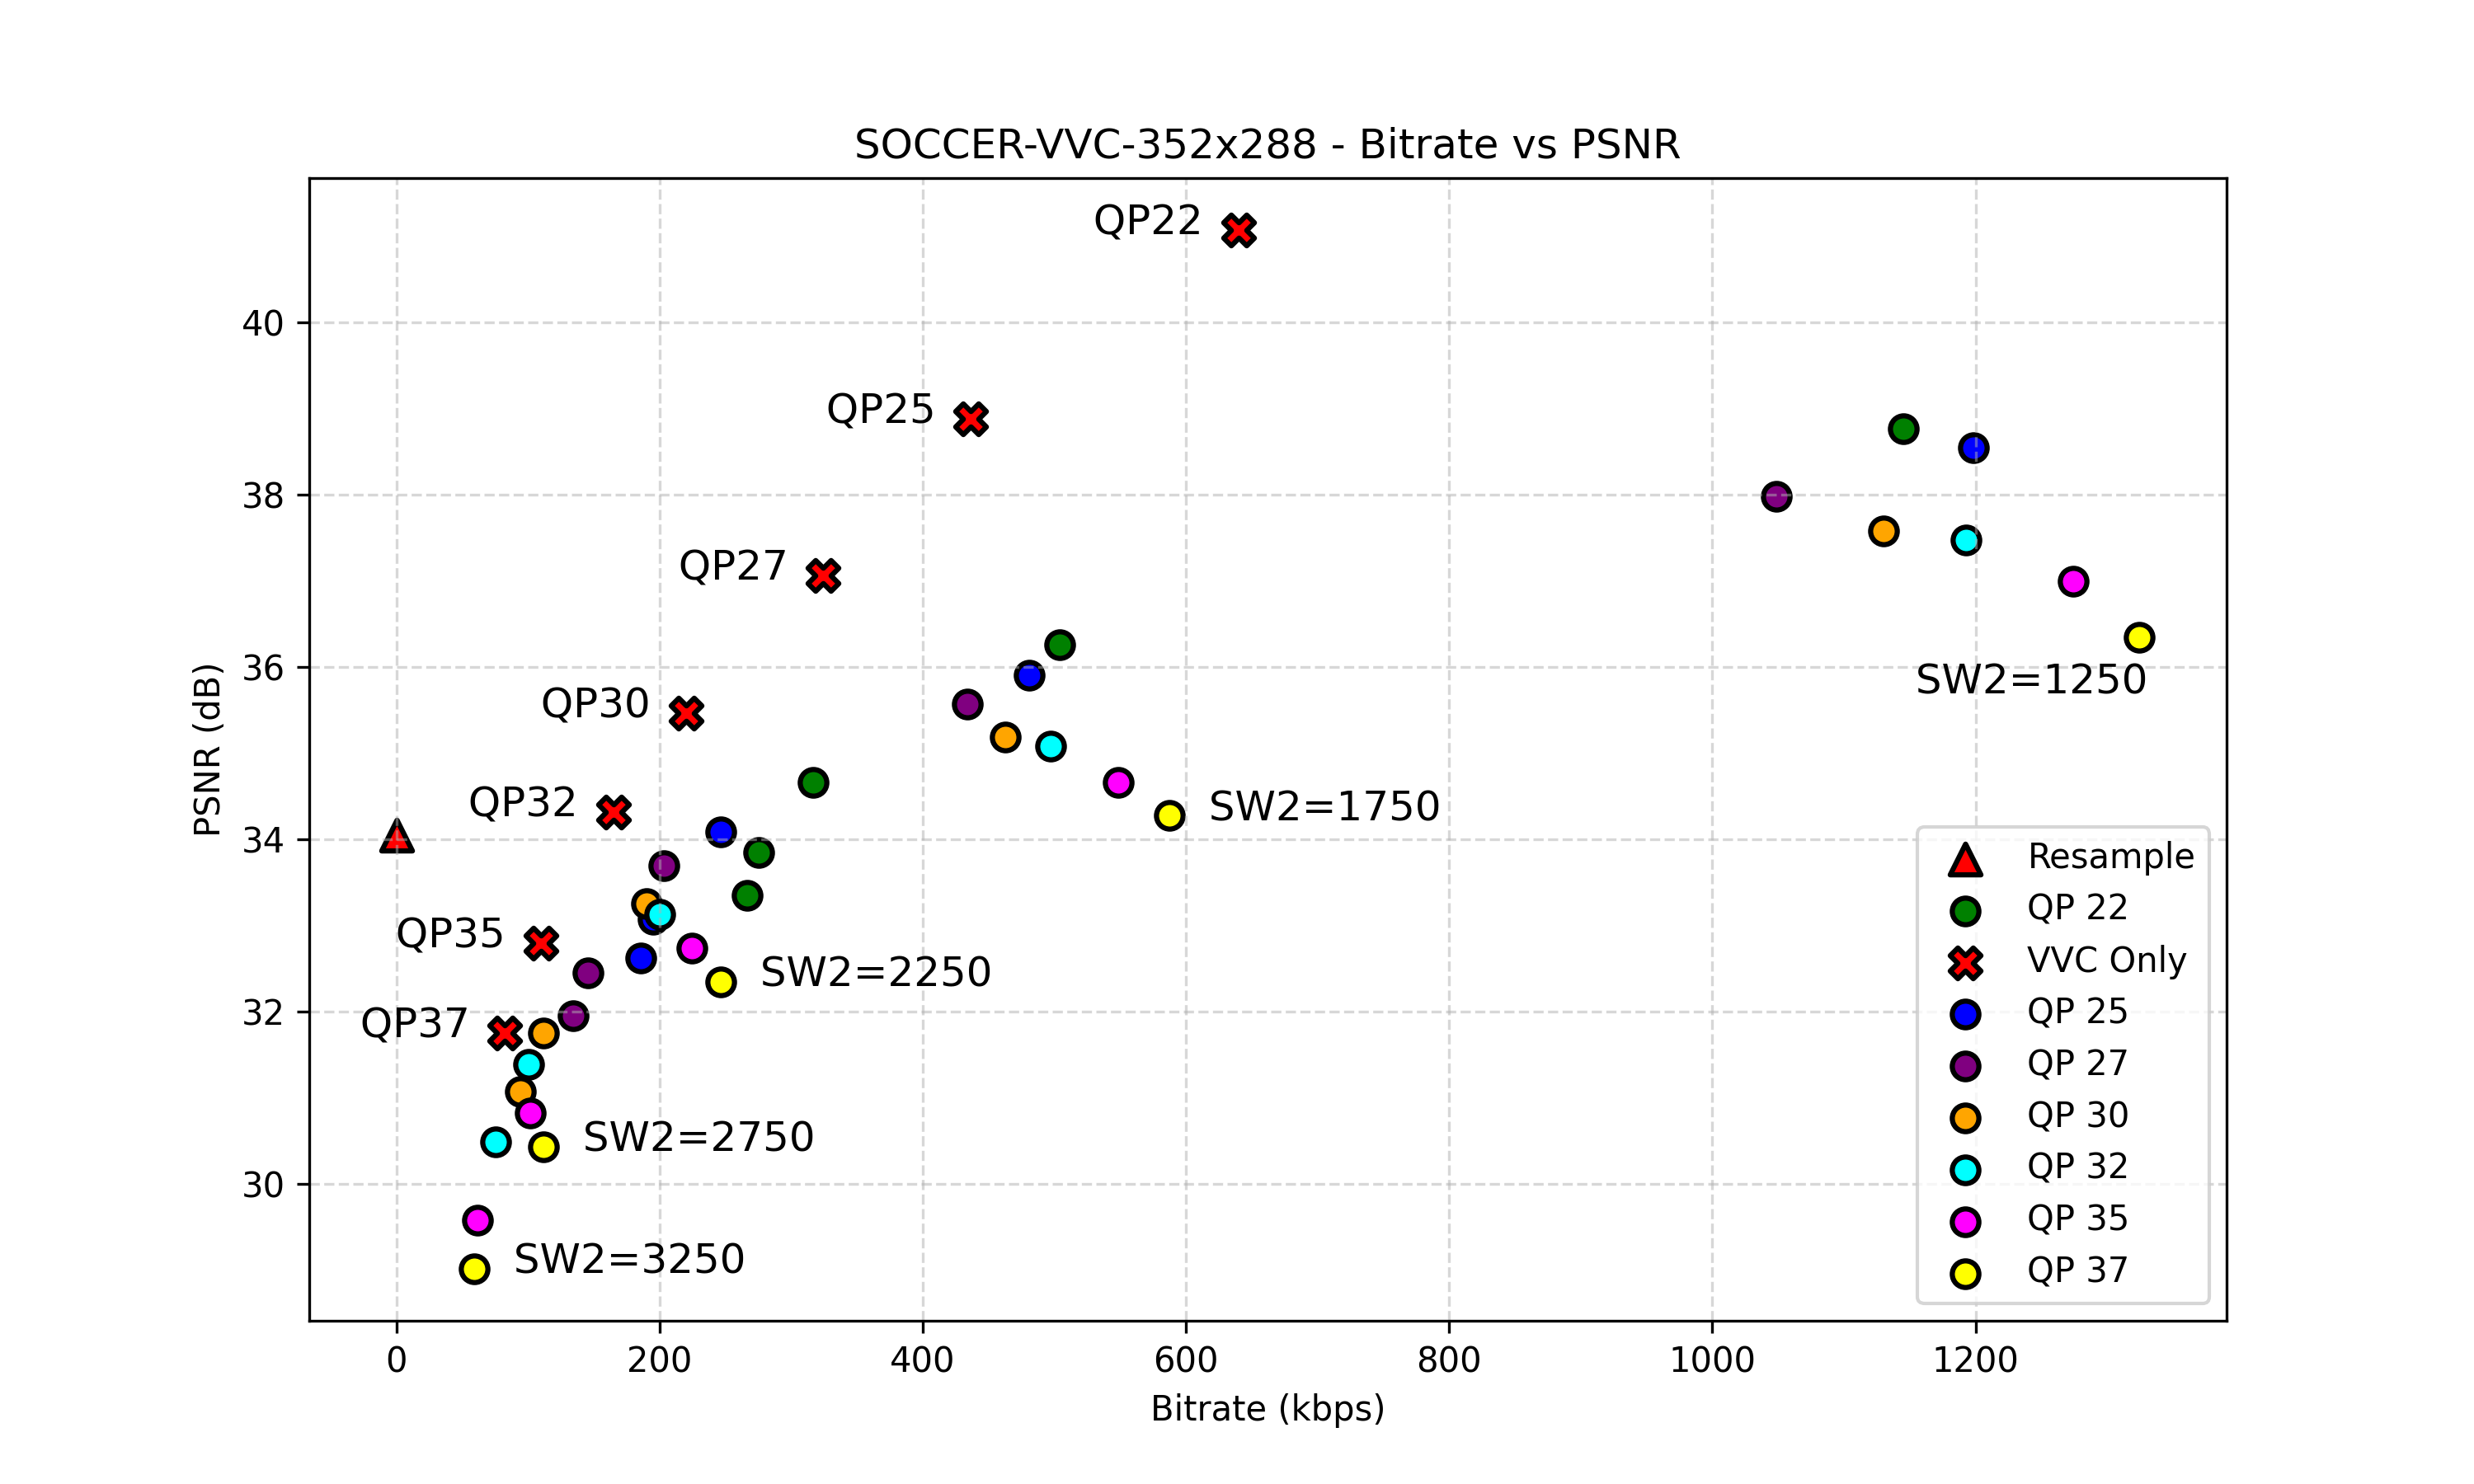
\includegraphics[width=1.0\textwidth]{img/SOCCER-VVC.png}
    \caption{Resultados para "SOCCER"\ em \acrshort{VVC}. \cite{xiph}}
    \label{fig:Soccer-VVC}
\end{figure}

Os resultados demonstram que neste caso houve uma vantagem para o uso de
somente o \acrshort{VVC}, com desempenho superior na maioria das configurações
avaliadas, principalmente em eficiência na relação qualidade e taxa.
Aqui a eficiência do \acrshort{LCEVC} foi abaixo do esperado, onde manteve
uma relação alta muita das vezes, indicando baixa eficiência na codificação
da camada base.

Nota-se que para valores de SW2 = 1250, os resultados demonstram um \textit{bitrate}
maior que o QP=22 do \acrshort{VVC} e um \acrshort{PSNR} muito inferior, tornando
estes resultados ineficientes.

O \textit{Resample} desta sequência também demonstrou um resultado ruim, atingindo
\acrshort{PSNR} menos que o QP=32 do \acrshort{VVC}.

Nesta sequência, o \acrshort{LCEVC} não apresentou vantagens, e muitas vezes
resultou no que seria uma perda de banda, sem ganhos significativos no
\acrshort{PSNR}.

\newpage
\subsection{Jockey}

\begin{figure}[h]
    \centering
    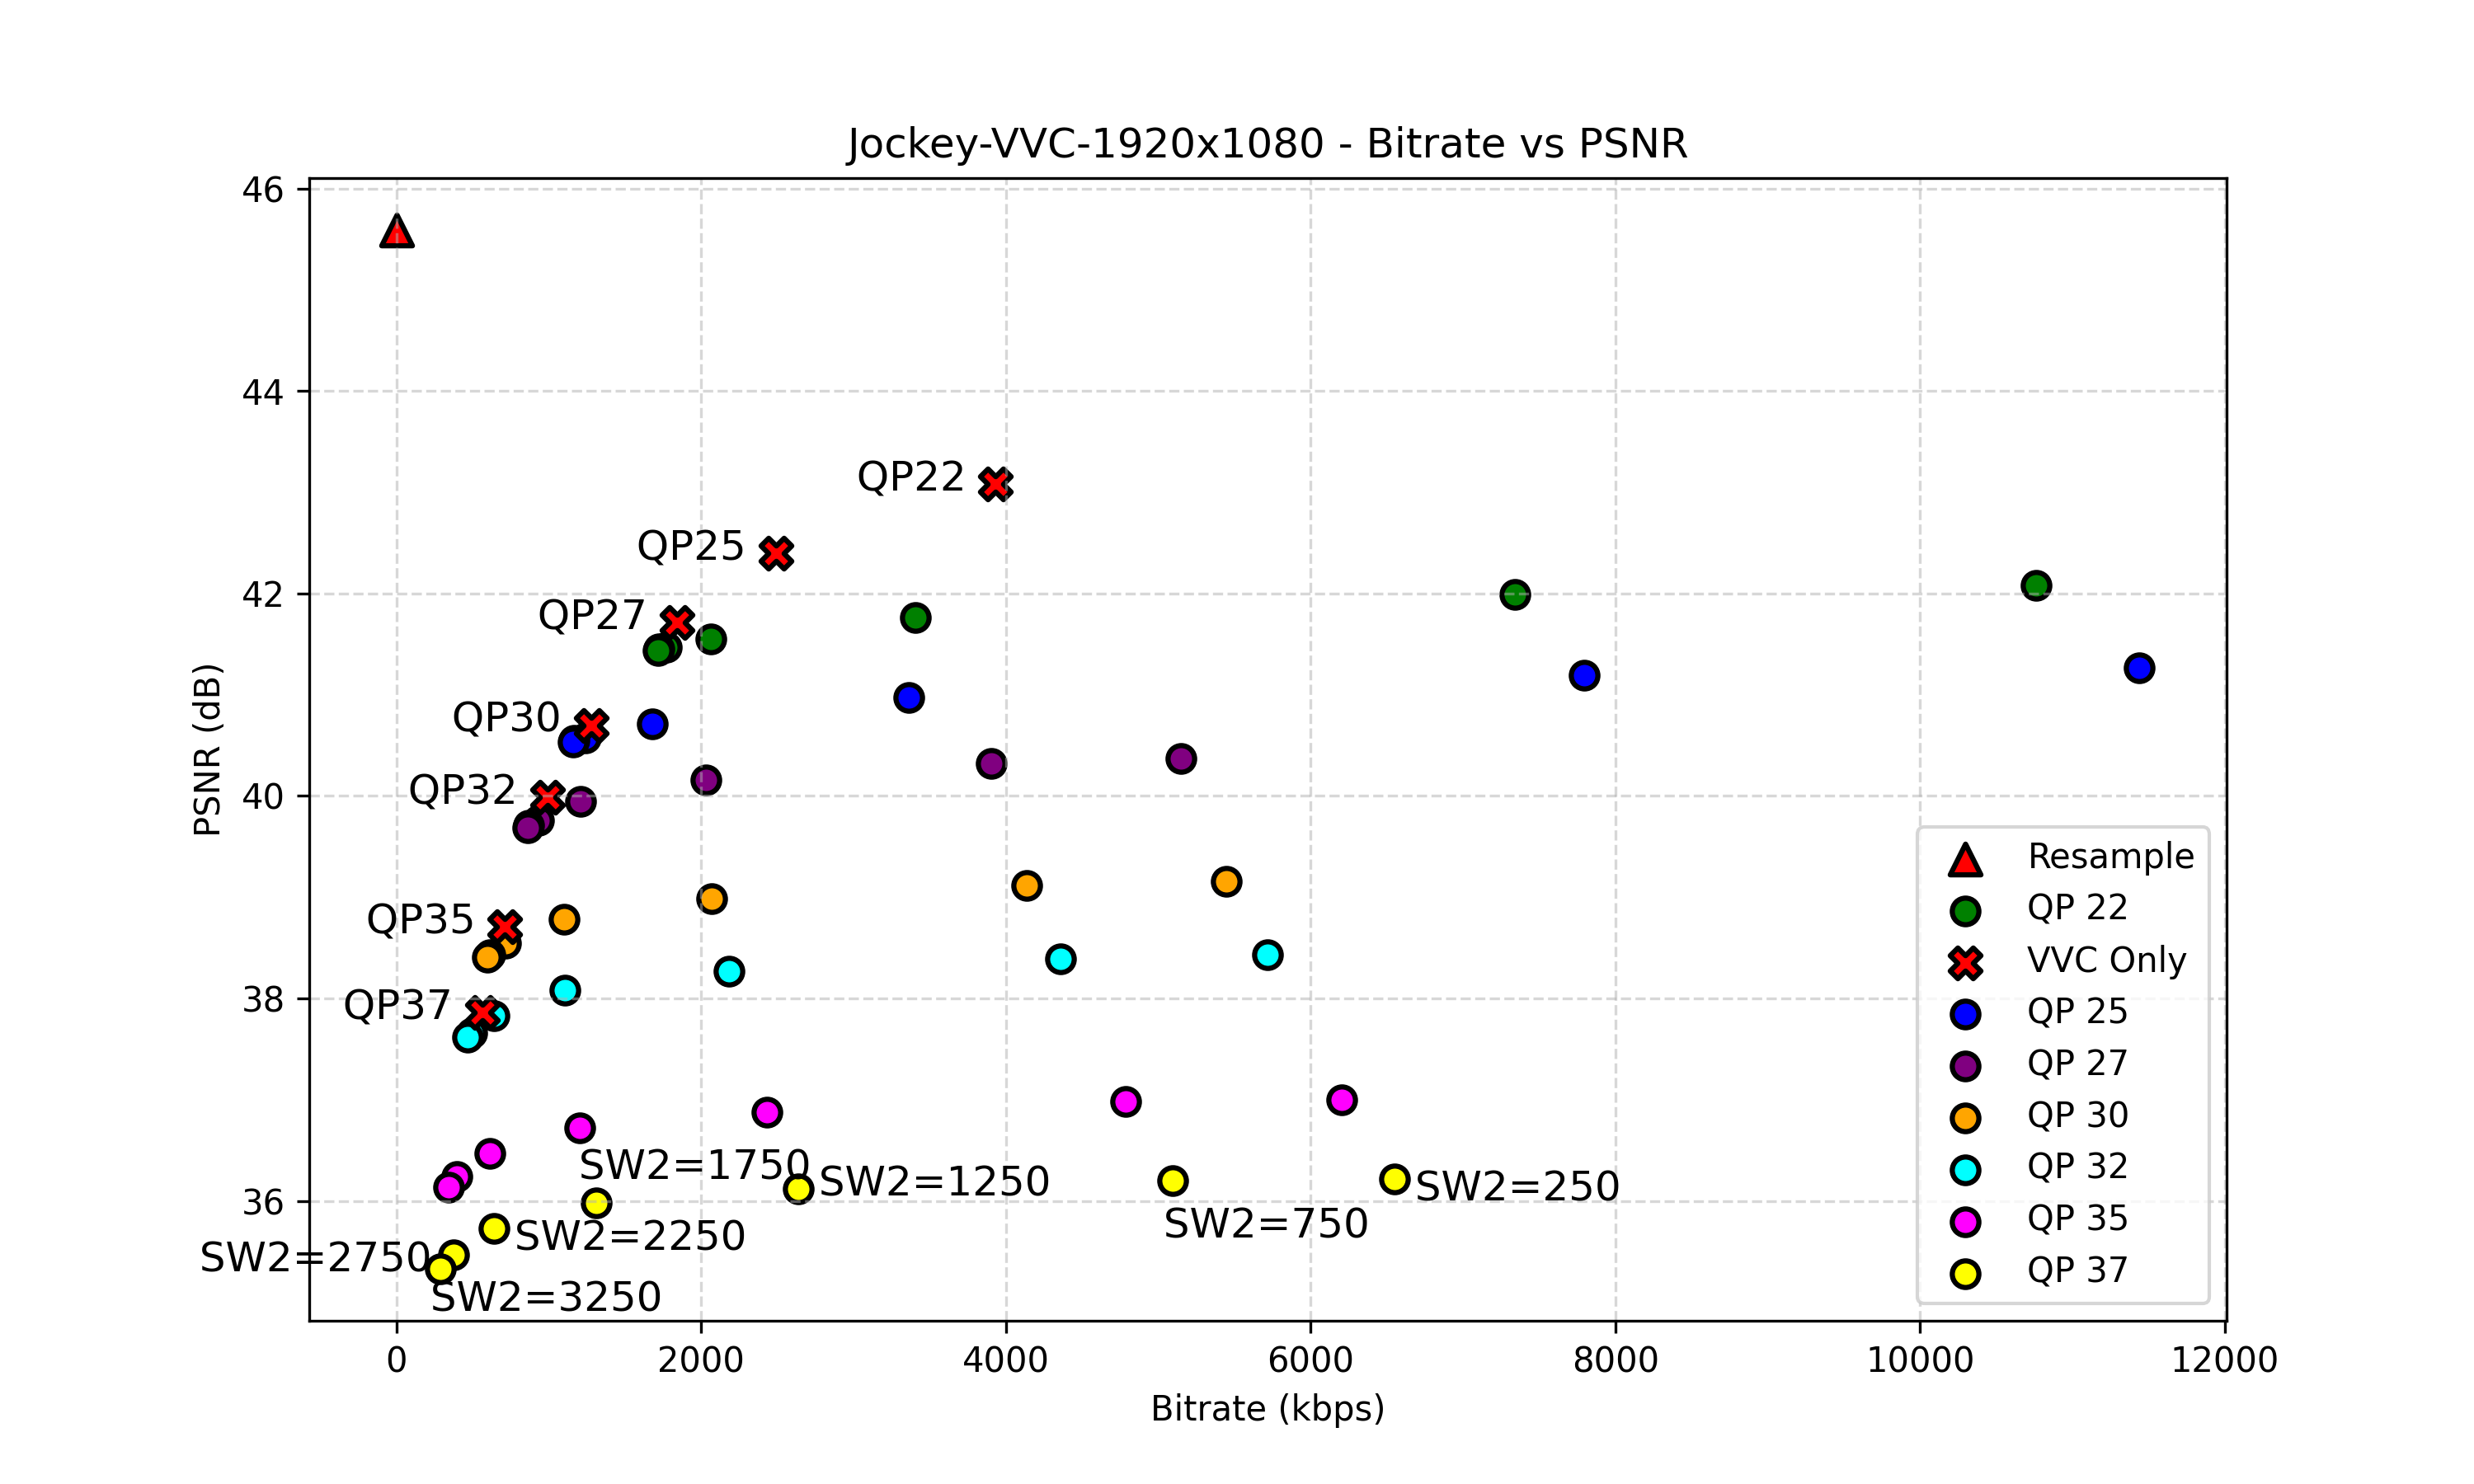
\includegraphics[width=1.0\textwidth]{img/Jockey-VVC.png}
    \caption{Resultados para "Jockey"\ em \acrshort{VVC}. \cite{uvg_dataset}}
    \label{fig:Jockey-VVC}
\end{figure}

A sequência "Jockey" apresentou resultados bastante equilibrados entre o uso do 
\acrshort{VVC} puro e o uso combinado do \acrshort{LCEVC}. Avaliando os  resultados
obtidos, observa-se que o desempenho do \acrshort{LCEVC} e \textit{bitrate} revela
que o desempenho do \acrshort{LCEVC}, neste caso, se aproxima consideravelmente do
\acrshort{VVC} isolado, e até melhor em alguns casos.

Para os resultados do \acrshort{LCEVC} com QPs iguais a 22 e 25, observou-se um 
comportamento incomum, onde o \textit{bitrate} destes pontos cresceram muito 
acima do esperado, saindo bastante da reta formada pelos pontos com o mesmo SW2.

Nesta sequência, a qualidade do \acrshort{LCEVC} se manteve consistente e próxima
dos valores obtidos por somente o uso do \acrshort{VVC}. Isso torna o uso do 
\acrshort{LCEVC} nesta sequência uma opção válida e demonstra ser uma alternativa
válida para casos de uso com vídeos semelhantes.

\newpage
\subsection{City}

\begin{figure}[h]
    \centering
    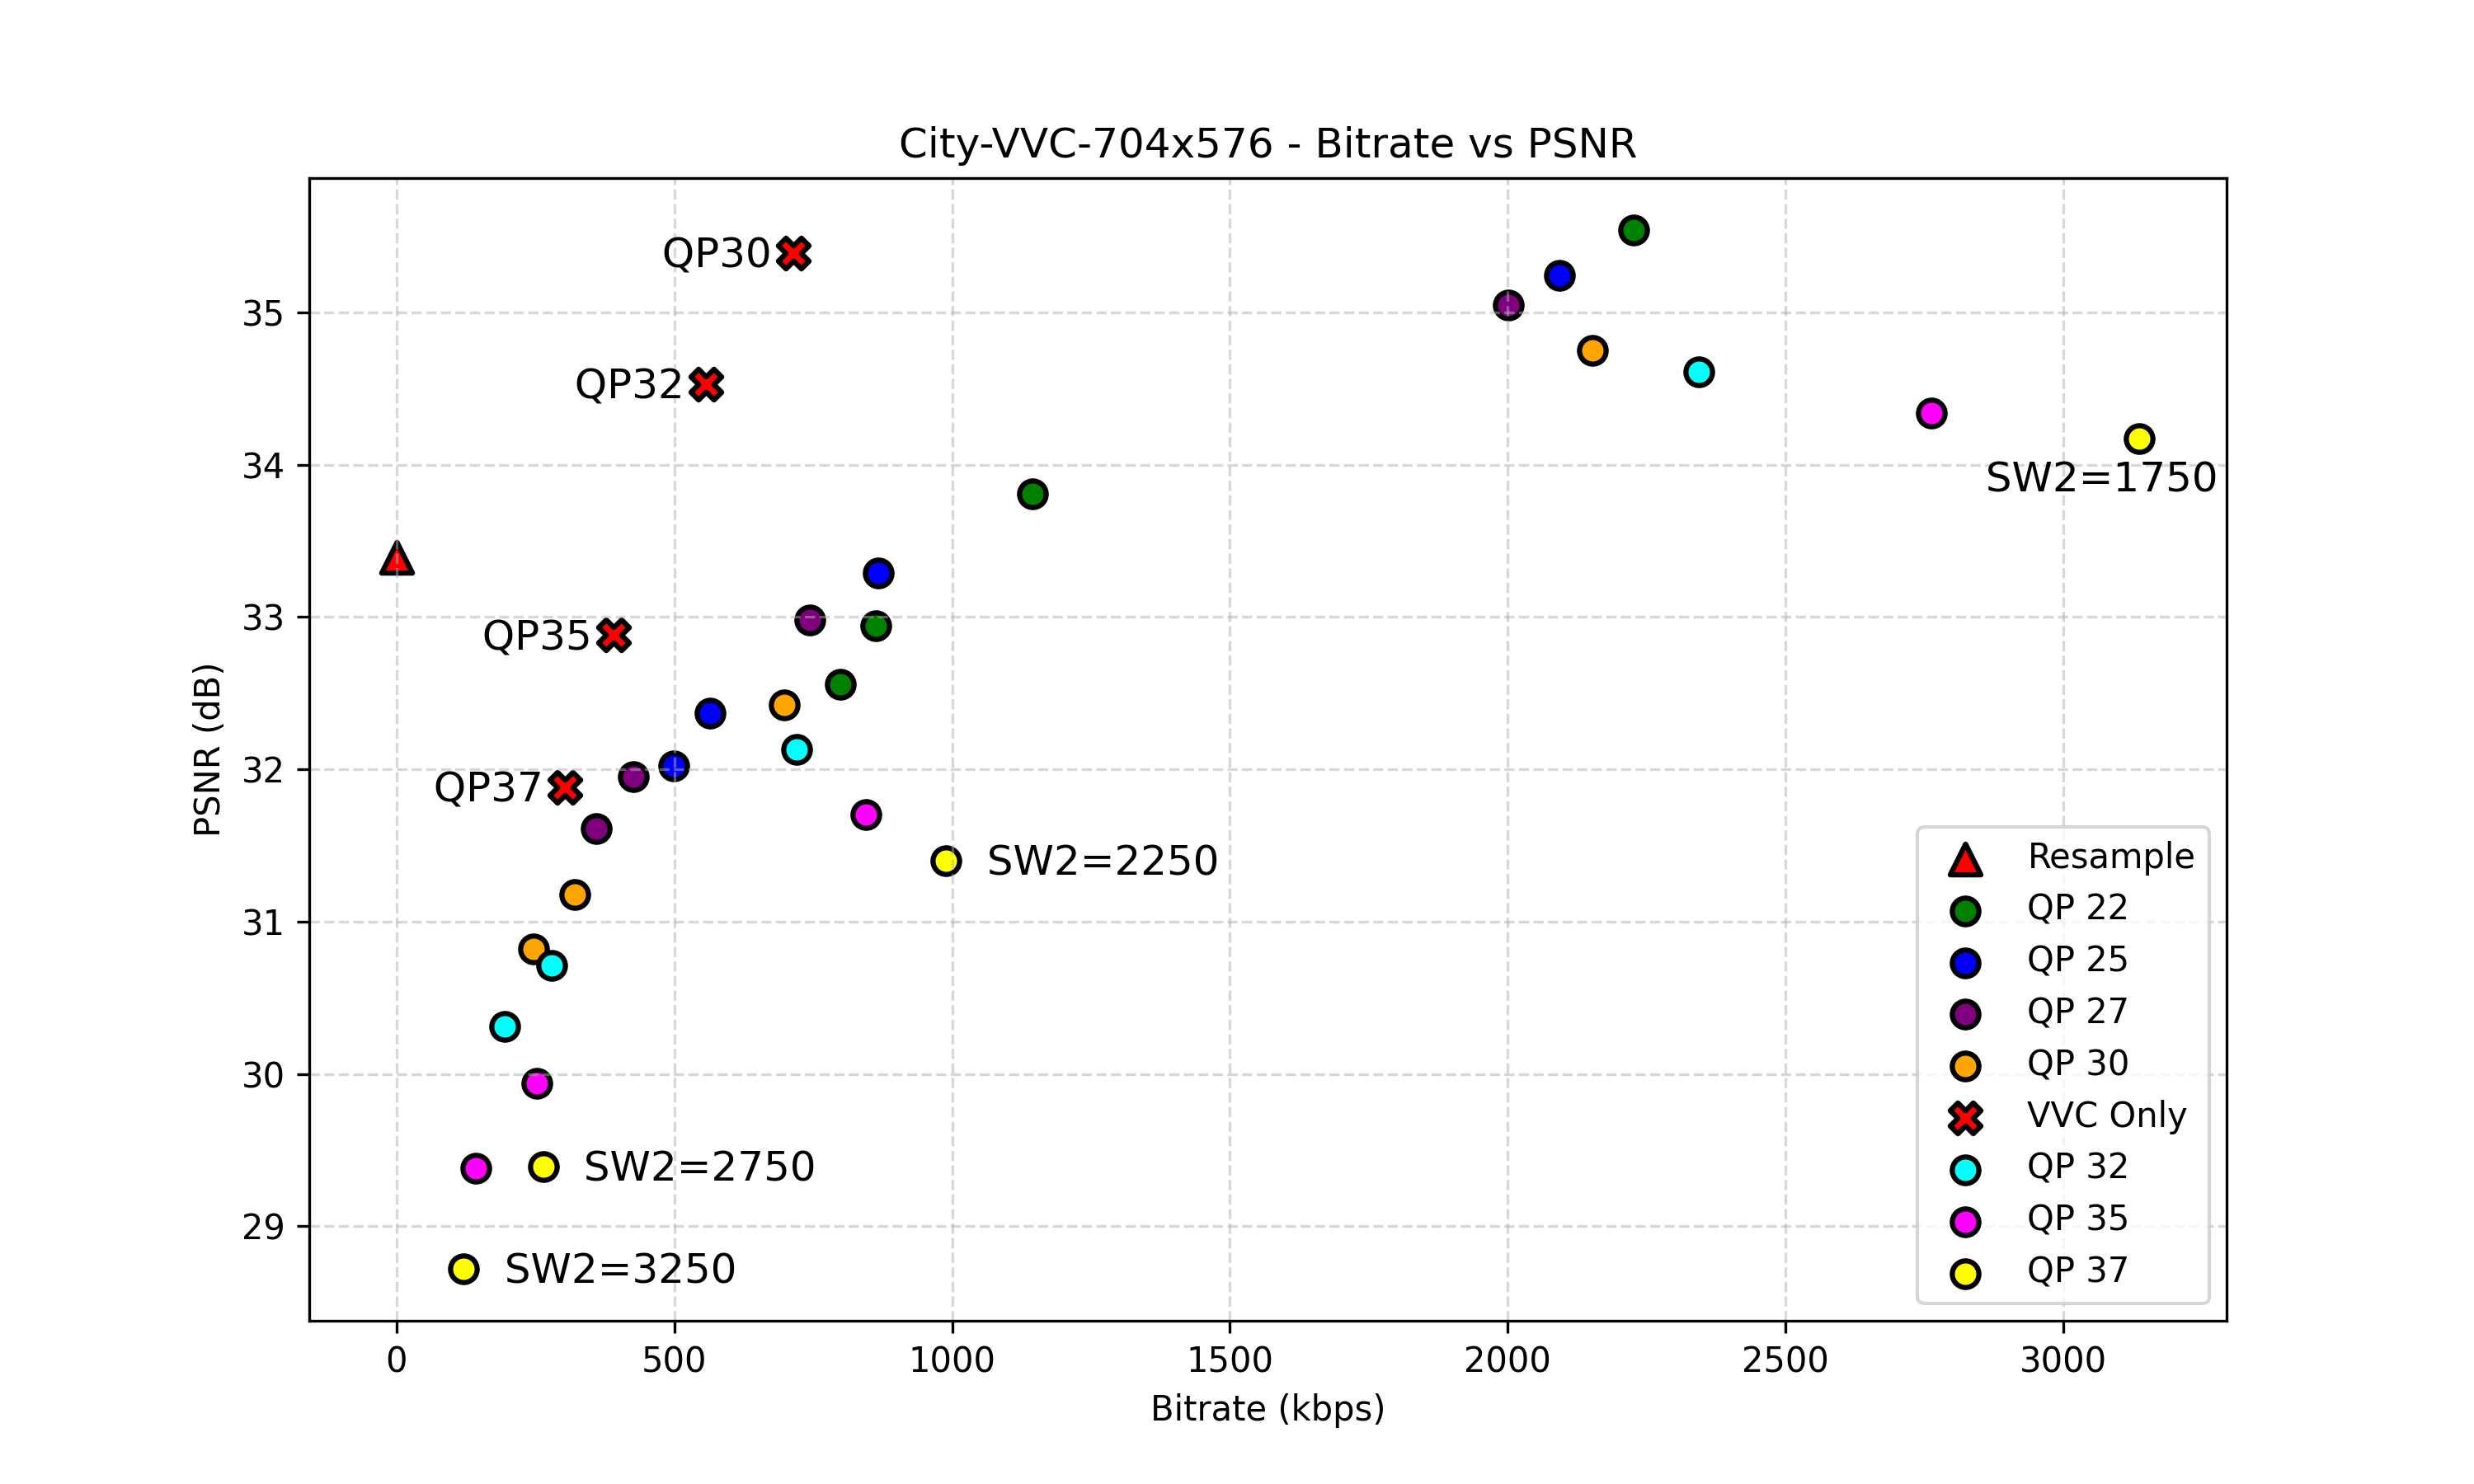
\includegraphics[width=1.0\textwidth]{img/City-VVC.png}
    \caption{Resultados para "City"\ em \acrshort{VVC}. \cite{xiph}}
    \label{fig:City-VVC}
\end{figure}

Na comparação \acrshort{VVC} puro e \acrshort{LCEVC} + \acrshort{VVC}, o desempenho
do \acrshort{VVC} isolado se mostrou eficiente. Esta sequência demonstra que o uso do
\acrshort{VVC} puro se mantém mais eficiente em praticamente todos os cenários testados.

Para o SW2 = 1750, os resultados do \acrshort{LCEVC} apresentaram um valor elevado para o
\textit{bitrate}. Todos os estes resultados estão acima de 2000 kbps de \textit{bitrate},
tornando estes resultados ineficientes em relação aos resto dos valores.


O \acrshort{LCEVC} não trouxe ganhos práticos para esta sequência, onde somente o
\acrshort{VVC} por si só foi mais eficiente e apropriado para codificação de sequências
como este vídeo aéreo de Nova York. 

Outro ponto interessante deste resultado é que o \textit{Resample} do \acrshort{LCEVC} obteve
uma qualidade inferior a vários pontos do \acrshort{VVC} puro e do \acrshort{LCEVC} + \acrshort{VVC}.


\newpage

\subsection{vc-philips-01}

\begin{figure}[h]
    \centering
    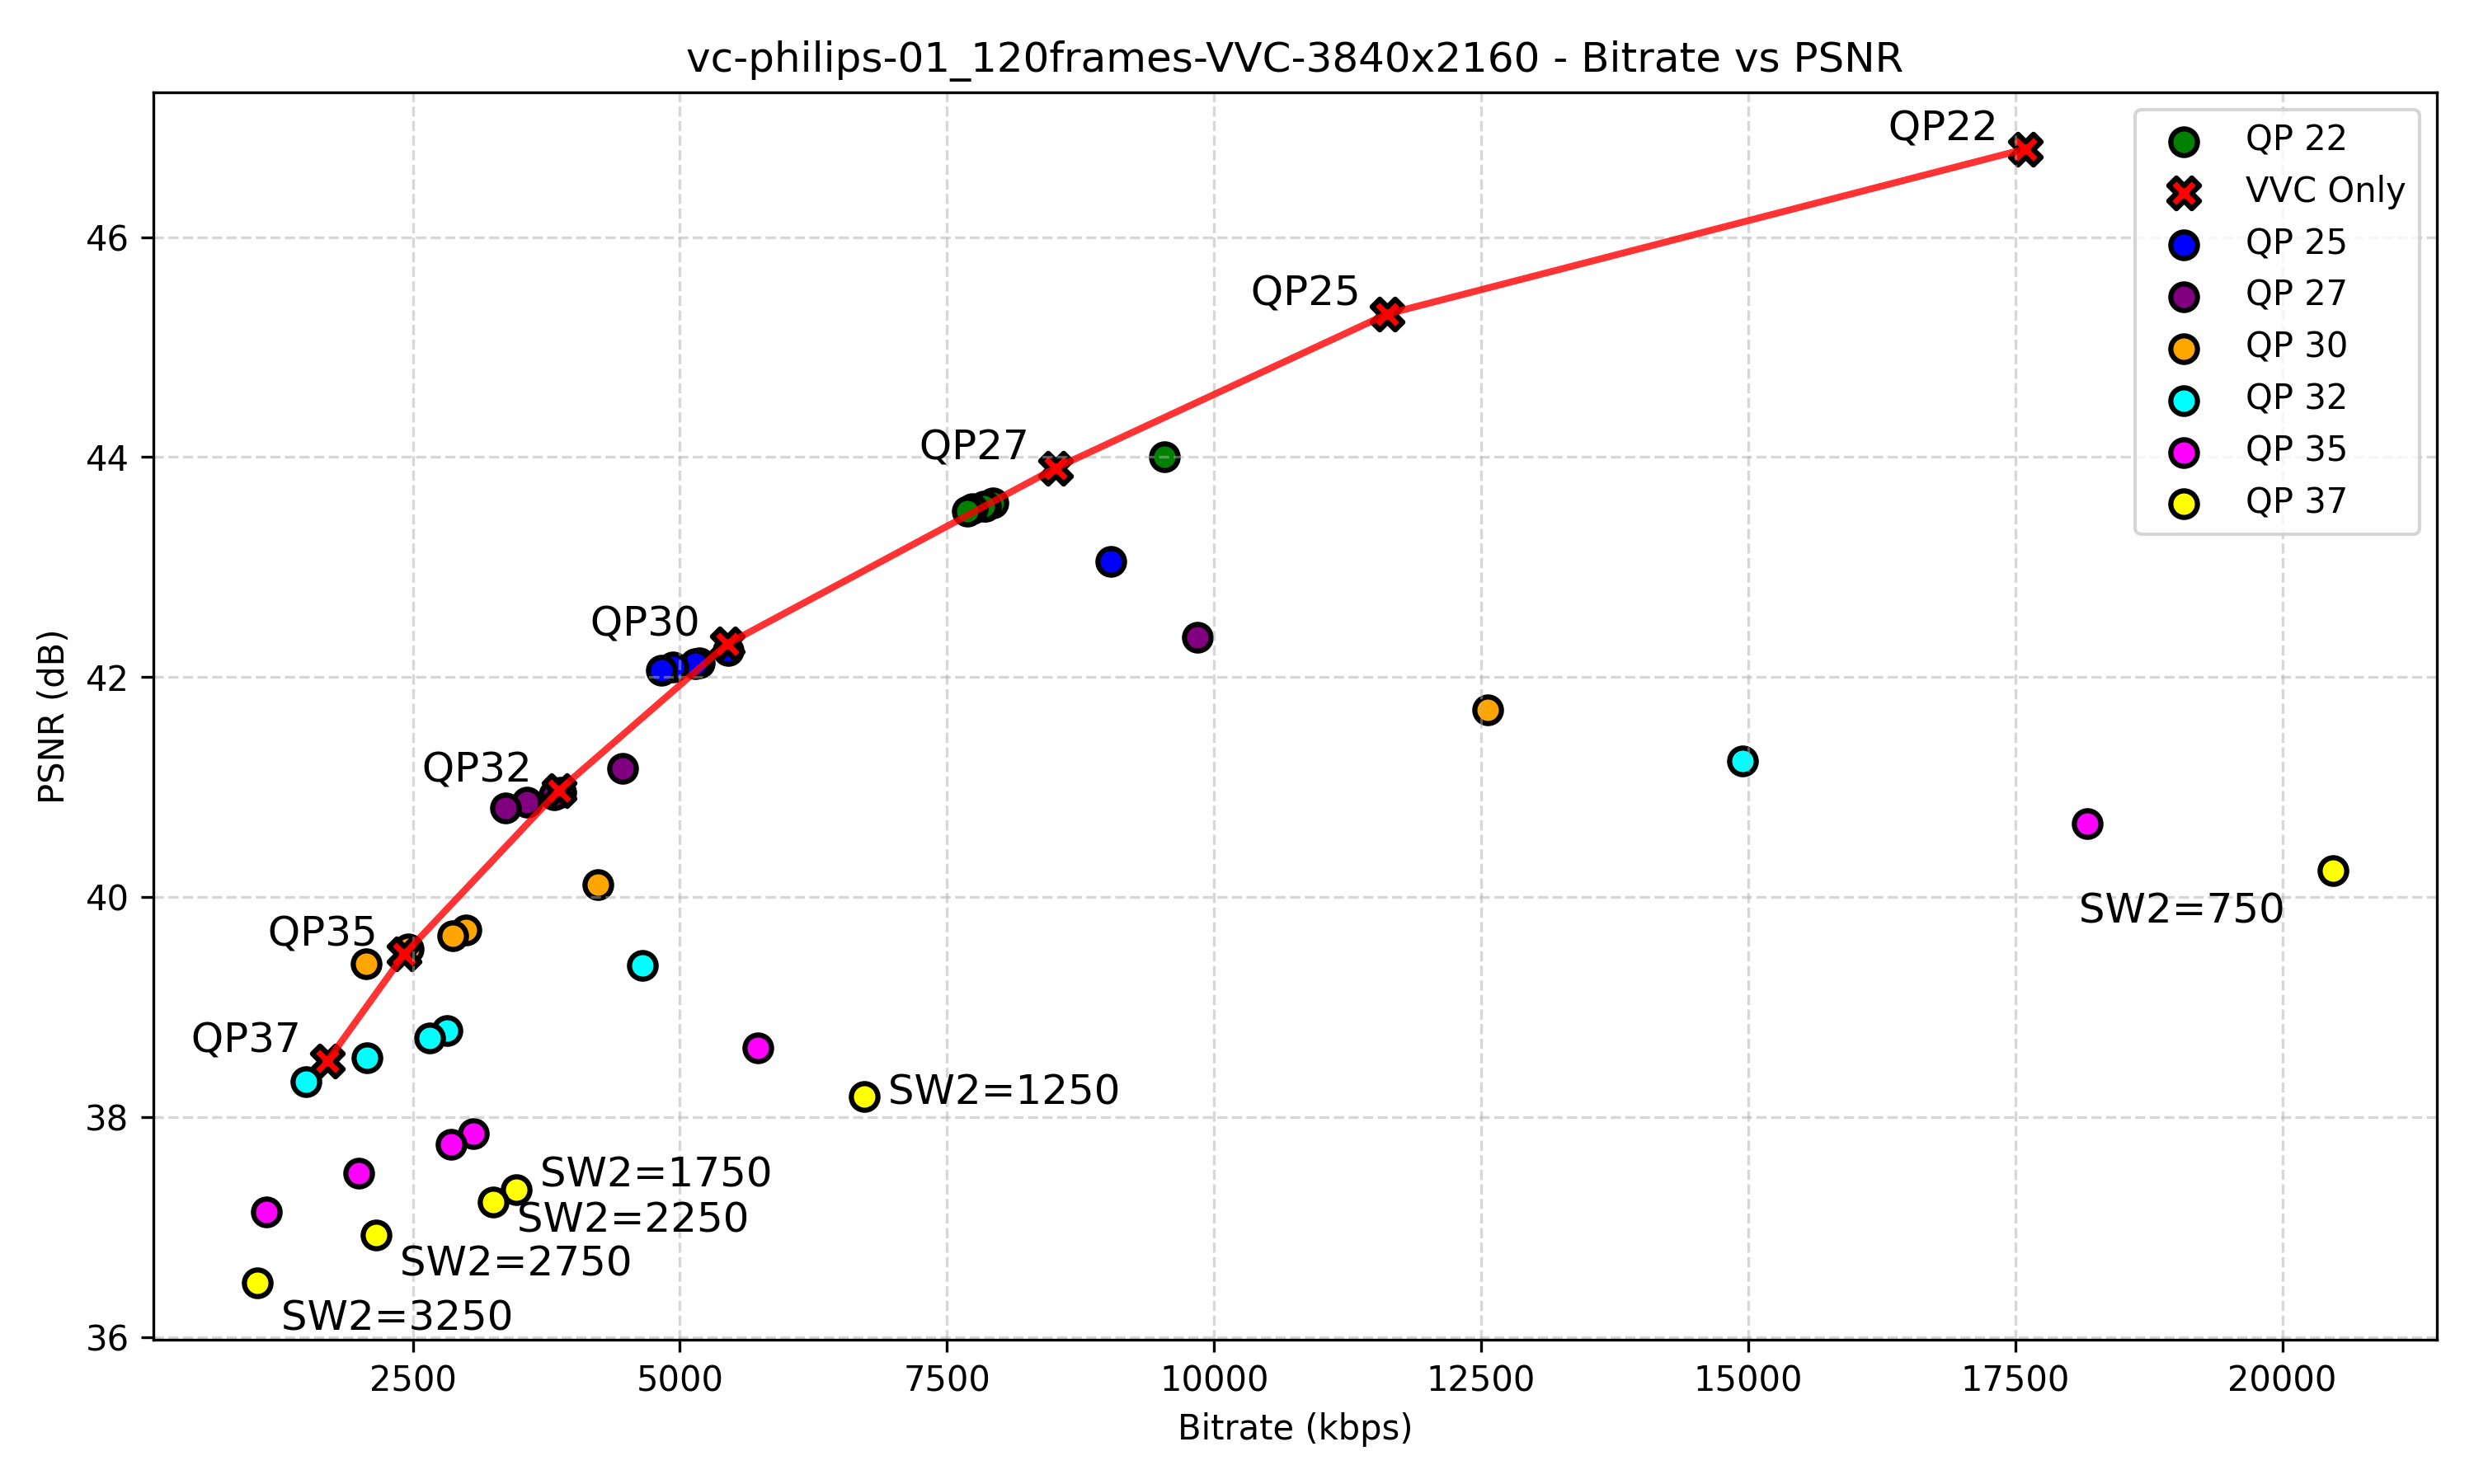
\includegraphics[width=0.5\textwidth]{img/vc-philips-01_120frames-VVC.png}
    \caption{Resultados para "vc-philips-01"\ em \acrshort{VVC}.}
    \label{fig:vc-philips-01-VVC}
\end{figure}

Nesta sequência, o SW2 = 750 obteve um \textit{bitrate} bem alto em relação ao
SW2 = 1250, onde também houve uma distância relativamente maior entre os valores de
QP dentro do SW2 = 750.

Em SW1= 1250, os pontos começaram a se aproximar da curva de eficiência, mas ainda 
assim com os valores abaixo da curva. O resto dos resultados para valores de SW2 menores
ficaram bem próximos e tendendo ao formato da curva do \acrshort{VVC}.

Conforme o valor de QP da base do \acrshort{LCEVC} foi diminuindo, mais próximos os 
resultados para tal QP foram ficando. Os resultados de QP igual a 22, 25 e 27, ficaram
muito próximos na maioria dos valores de SW2. Como as proporções da camada de aprimoramento
destes valores ficaram entre 0,2\% e 3,2\%, isto afetou a eficiência do \acrshort{LCEVC}, que
ficou mais perceptível em uma sequência em 4K.

O \acrshort{LCEVC} conseguiu alcançar ótimos resultados, onde vários pontos estiveram
acima da curva de eficiência do \acrshort{VVC}, entrando para a fronteira de Pareto.

\newpage

\subsection{vc-globo-05}

\begin{figure}[h]
    \centering
    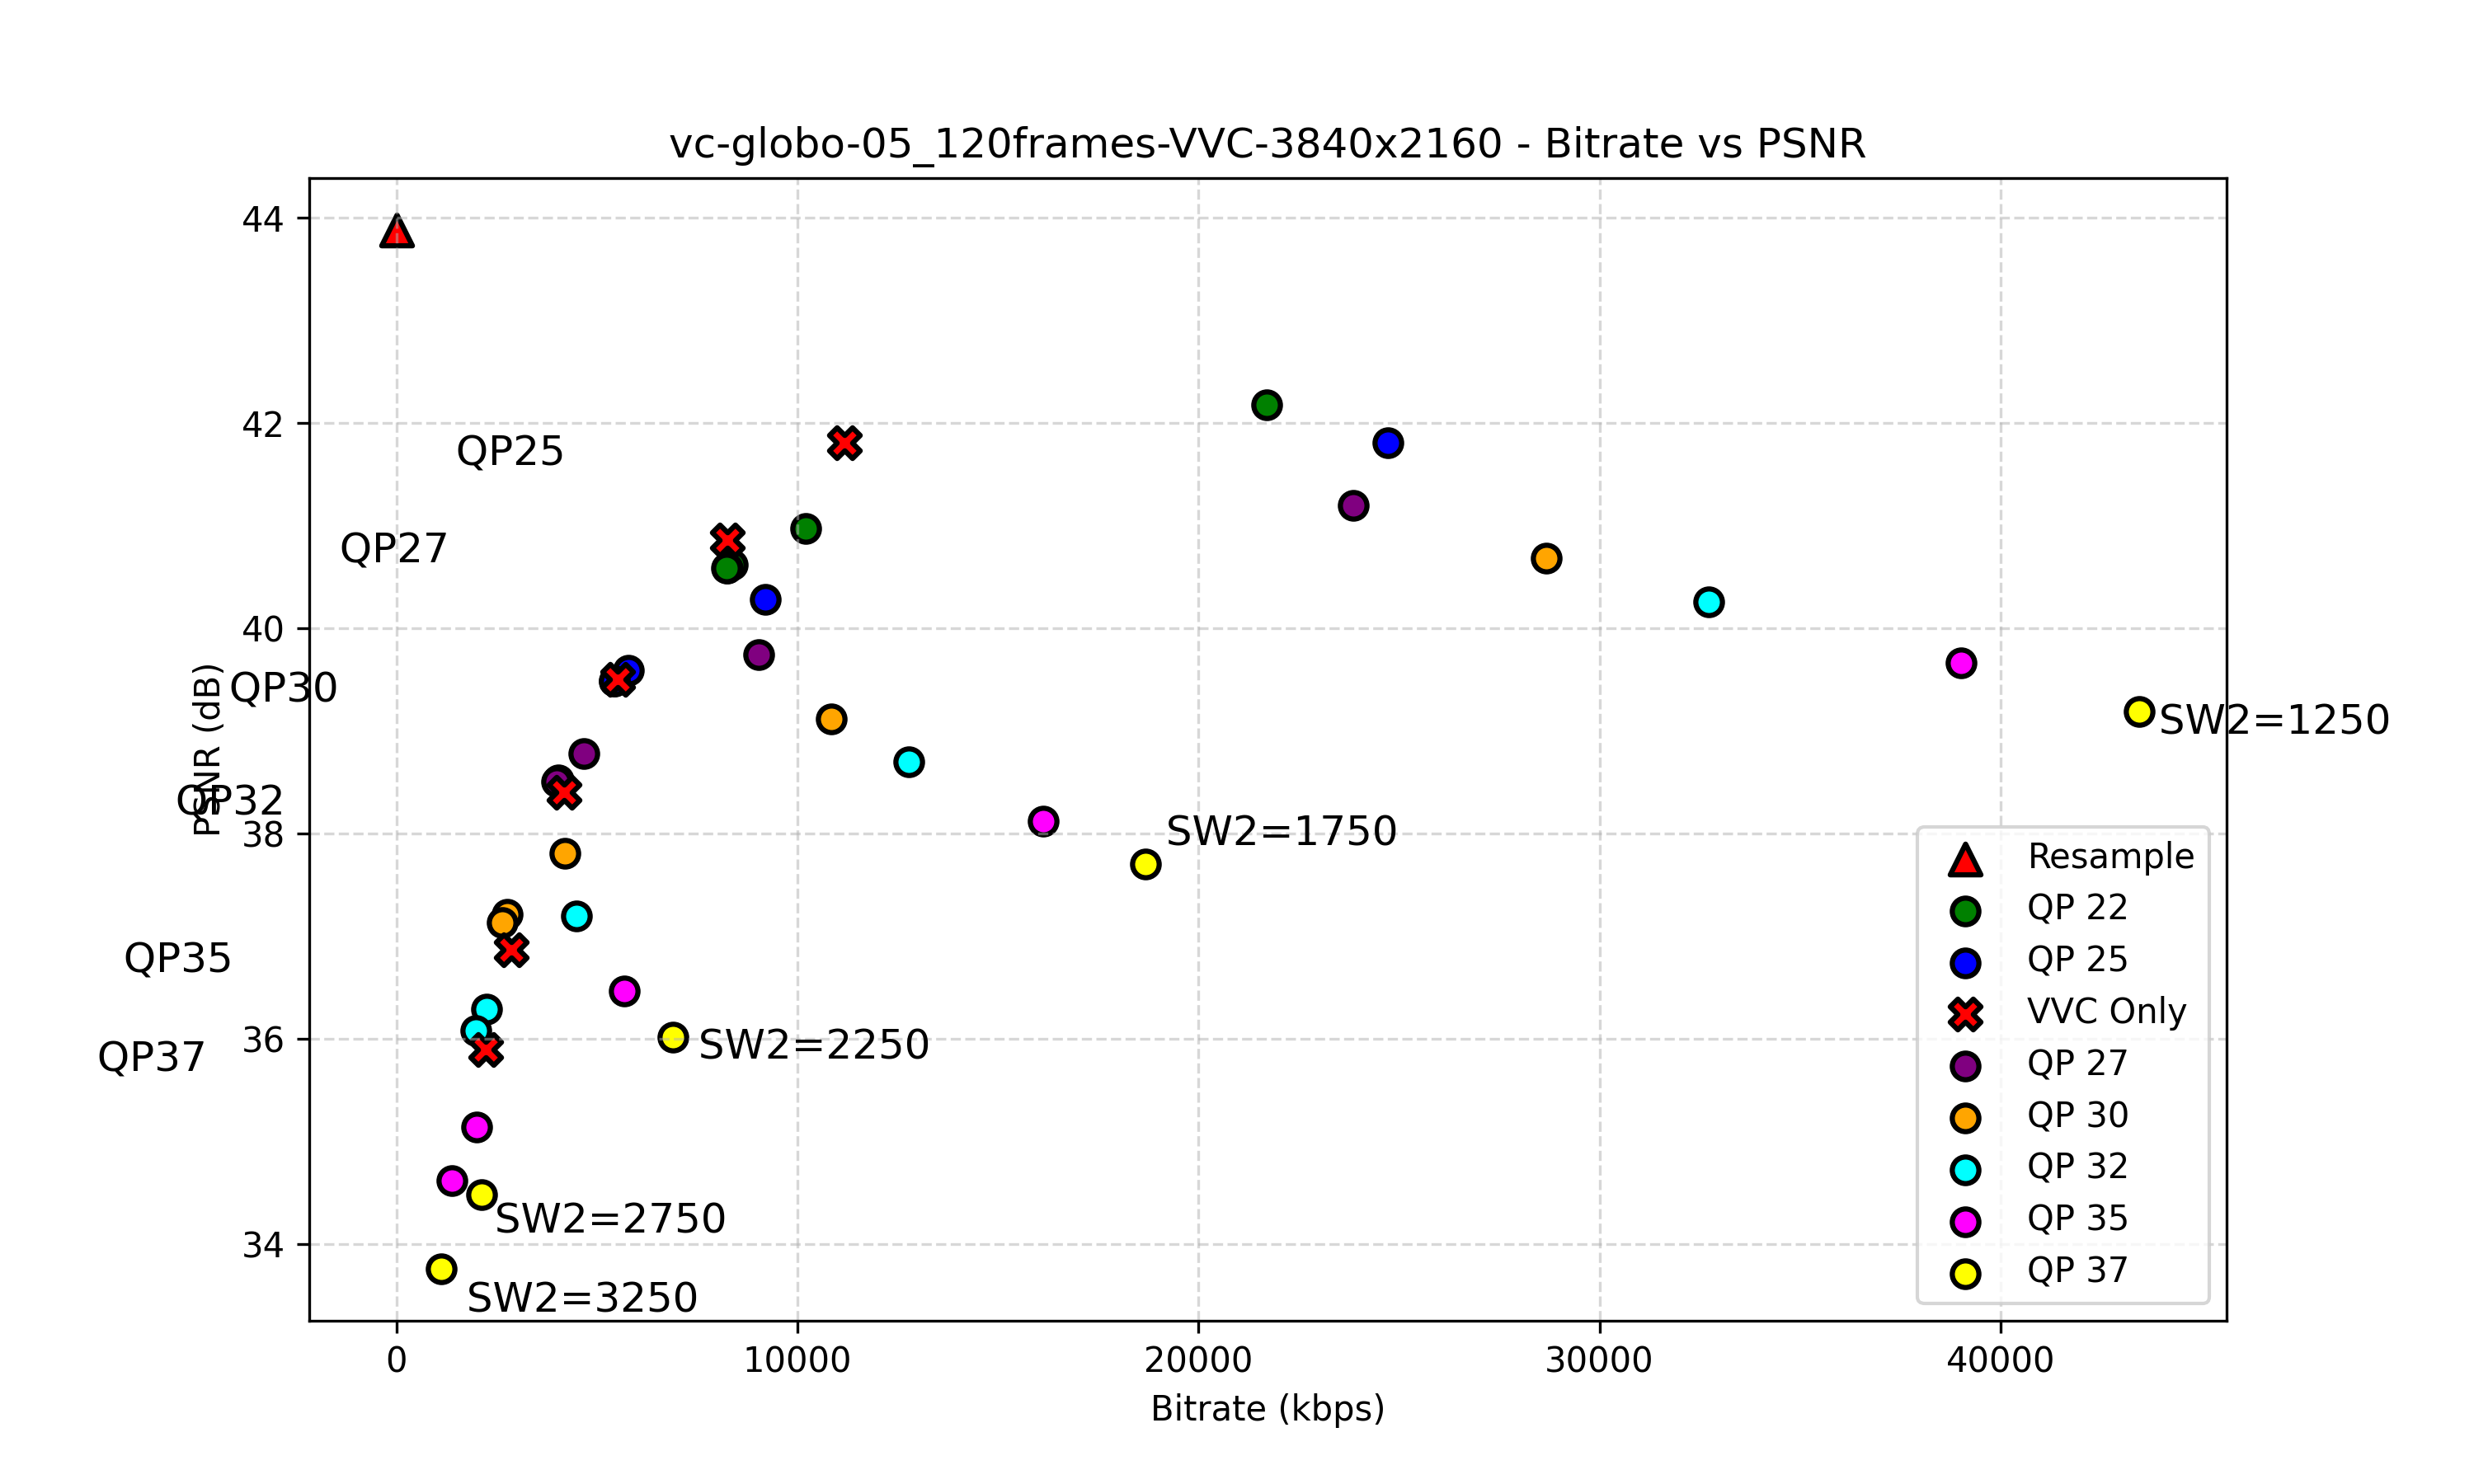
\includegraphics[width=1.0\textwidth]{img/vc-globo-05_120frames-VVC.png}
    \caption{Resultados para "vc-globo-05"\ em \acrshort{VVC}.}
    \label{fig:vc-globo-05-VVC}
\end{figure}

Os resultados os vídeos gerados com o \acrshort{LCEVC} e \acrshort{VVC} alcançaram
um desempenho similar, onde há vários pontos na curva de melhor qualidade tanto 
do \acrshort{LCEVC} quanto do \acrshort{VVC}. Os resultados para valores mais baixos
de SW2 continuam com uma diferença grande de \textit{bitrate} entre eles.

No ponto QP =25 e SW2 = 1250, o \acrshort{LCEVC} alcançou um \acrshort{PSNR} de 41,81 db
a 24,7 Mbps, exatamente o mesmo valor do \acrshort{VVC} com QP = 25, porém com um
\textit{bitrate} maior que o sobro da solução base de somente o \acrshort{VVC}, que
obteve um \textit{bitrate} de 11,1 Mbps.

O resultados do \acrshort{LCEVC} com QP = 32 e 30, foram ligeiramente superiores
aos resultados do \acrshort{VVC}, onde o \textit{bitrate} foi menor e o \acrshort{PSNR} foi
superior. Na prática, esta vantagem é imperceptível, mas demonstra que o \acrshort{LCEVC}
pode ser vantajoso em alguns casos.

\newpage

\section{Considerações}

\begin{itemize}
    \item O comportamento do \acrshort{LCEVC} varia conforme a sequência testada, o
    que é esperado, já que o padrão atua como uma camada adaptativa;

    \item O \acrshort{LCEVC} demonstrou um desempenho superior em sequências que
    envolvam mais movimentação de câmera e detalhes, como no caso da sequência "Jockey";
    
    \item A vantagem do \acrshort{LCEVC}  se mostra mais evidente em cenários de
    \textit{bitrate} mais restrito, onde o refinamento da imagem se torna crucial;

    \item Em taxas mais altas, o benefício da camada de aprimoramento tende a diminuir,
    pois a camada base já está oferecendo uma boa qualidade;

    \item Também é importante observar que o uso do \acrshort{LCEVC} com codecs mais
    simples, como o \acrshort{AVC} tende a ser mais vantajoso do que com outros codecs
    mais avançados, como o \acrshort{VVC}, uma vez que o ganho sobre algo já bem
    otimizado costuma ser menor;

    \item Nos testes realizados, foi possível observar que mesmo quando há uma proporção
    bem alta para a camada de aprimoramento, o ganho de \acrshort{PSNR} não é direto, onde
    muitos casos o \textit{bitrate} do \acrshort{LCEVC} é muito maior que um vídeo utilizando
    somente o codificador base, e a qualidade aferida pelo \acrshort{PSNR} é muito menor.
\end{itemize}

\newpage
\section{Visão geral dos resultados}

Após a análise de cada sequência, foi feito uma interpretação dos resultados e definido
qual deles se saiu melhor no geral. Vale ressaltar que mesmo que um tipo de codificação
tenha se saído melhor, como a maioria dos resultados foram muito próximos, pode não haver
uma diferença significativa na qualidade visual ou tamanho. Foram considerados somente os
pontos que estão próximos da curva de eficiência (Fronteira de Pareto).

\begin{table}[h]
    \centering
    \begin{tabular}{|c|c|}
        \hline
        \textbf{Sequência} & \textbf{Resultado}\\
        \hline
        Bosphorus (1920x1080, AVC) & Leve vantagem para o LCEVC\\
        \hline
        ReadySteadyGo (1920x1080, AVC) & Vantagem para o AVC\\
        \hline
        Jockey (1920x1080, AVC) & Vantagem para o LCEVC\\
        \hline
        SOCCER (352x288, AVC) & Vantagem para o AVC\\
        \hline
        City (704x576, AVC) & Vantagem para o AVC\\
        \hline
        vc-globo-05 (3840x2160, AVC) & Empate\\
        \hline
        vc-lcevc-01 (3840x2160, AVC) & Empate\\
        \hline
        vc-philips-01 (3840x2160, AVC) & Empate\\
        \hline
        vc-philips-03 (3840x2160, AVC) & Leve vantagem para o LCEVC\\
        \hline
    \end{tabular}
    \caption{Compilado dos resultados finais para AVC.}
    \label{tab:results-avc}
\end{table}

\begin{table}[h]
    \centering
    \begin{tabular}{|c|c|}
        \hline
        \textbf{Sequência} & \textbf{Resultado}\\
        \hline
        Bosphorus (1920x1080, VVC) & Empate\\
        \hline
        SOCCER (352x288, VVC) & Vantagem para o VVC\\
        \hline
        Jockey (1920x1080, VVC) & Empate\\
        \hline
        City (704x576, VVC) & Empate\\
        \hline
        vc-globo-05 (3840x2160, VVC) & Leve vantagem para o LCEVC\\
        \hline
        vc-lcevc-01 (3840x2160, VVC) & Vantagem VVC\\
        \hline
        vc-philips-01 (3840x2160, VVC) & Leve vantagem para o LCEVC\\
        \hline
    \end{tabular}
    \caption{Compilado dos resultados finais do VVC.}
    \label{tab:results-vvc}
\end{table}